\documentclass[12pt]{amsart}

%Lots of packages :P
\usepackage[margin=1in]{geometry}  %1 inch margins
\usepackage{graphicx, array, blindtext}
\usepackage{amsthm, amsmath, amssymb,tikz, caption, subcaption}
\usepackage{comment}
\usepackage{multirow}%allows a table cell to span multiple rows
\usepackage{longtable}%allows tables to span multiple pages
\usepackage{booktabs}%for \cmidrule
\usepackage{caption, subcaption}%for messing with captions
\usepackage{enumitem}

\usetikzlibrary{calc}

%vertex styles
\tikzstyle{vx}=[shape=circle, minimum size=2mm, inner sep=0, fill=black]
\tikzstyle{whitevx}=[shape=circle, minimum size=2mm, draw=black, thick, fill=white, inner sep=0]%formerly red
\tikzstyle{grayvx}=[shape=circle, minimum size=2mm, draw=black, thick, dash pattern = on 2pt off 1 pt, fill=gray!90, inner sep=0]%formerly blue


%edge styles
\tikzstyle{grayedge}=[line width=2.5pt,dash pattern=on 1pt off 1pt]
\tikzstyle{sgrayedge}=[line width=1.875pt,dash pattern=on 1pt off 1pt]
\tikzstyle{emphedge}=[ultra thick, dotted]


\usepackage{float}%can force table location, need \begin{table}[H] instead of [htdp]
\restylefloat{table}

%for table of contents with links:
\usepackage{color}
\usepackage{hyperref}
\hypersetup{
    colorlinks=true, %set true if you want colored links
    linktoc=all,     %set to all if you want both sections and subsections linked
    linkcolor=blue,  %choose some color if you want links to stand out
    filecolor=green
}

\usepackage{listings} %For pretty programming code
\lstset{language=Python}

\usepackage[toc,page]{appendix} %yay, appendices!

\usepackage{todonotes} % todo comments
\usepackage{xspace}
%\usepackage{tabu}
\usepackage{bigstrut}

%Theorems
\theoremstyle{plain}
\newtheorem{thm}{Theorem}[section]
\newtheorem{lem}[thm]{Lemma}
\newtheorem{lemma}[thm]{Lemma}
\newtheorem{prop}[thm]{Proposition}
\newtheorem{claim}[thm]{Claim}
\newtheorem{conj}[thm]{Conjecture}
\newtheorem{cor}{Corollary}[thm]


\theoremstyle{definition}
\newtheorem{defn}[thm]{Definition}
\newtheorem{obs}[thm]{Observation}
\newtheorem{ques}[thm]{Question}
\newtheorem{cons}[thm]{Construction}

\theoremstyle{remark}
\newtheorem*{rmk}{Remark}
\newtheorem{case}{Case}[thm]
\newtheorem{subcase}{Subcase}[case]


%Commands
\newcommand{\indsat}[2]{\ensuremath{\operatorname{indsat}(#1,#2)}\xspace}
\newcommand{\sis}[2]{\ensuremath{{\operatorname{indsat}}^*(#1,#2)}\xspace}
\newcommand{\sat}[2]{\ensuremath{\operatorname{sat}(#1,#2)}\xspace}
\newcommand{\ex}[2]{\ensuremath{\operatorname{ex}(#1,#2)}\xspace}

\newcommand{\claw}{\ensuremath{K_{1,3}}\xspace}
\newcommand{\paw}{\ensuremath{K_{1,3}^+}\xspace}

\newcommand{\Km}{$K^{(t_1,\ldots,t_{i-1})}$}
\newcommand{\Kk}{$K^{(t_1,\ldots,t_{k-1})}$}

%use this for referencing, in the submitted toggle, the arxiv version.
\newcommand{\arxiv}{www.arxivurl.edu}

\renewcommand{\bar}{\overline}

\newcommand{\cl}[1]{\lceil#1\rceil}
\newcommand{\CL}[1]{\left\lceil#1\right\rceil}
\newcommand{\fl}[1]{\lfloor#1\rfloor}
\newcommand{\FL}[1]{\left\lfloor#1\right\rfloor}

\newcommand{\cartprod}{\mathop{\scriptsize\Box}}


%for toggling
\usepackage{etoolbox}

\providetoggle{sub}
\settoggle{sub}{false}
\providetoggle{todo}
\settoggle{todo}{true}
\newtoggle{edit}
\togglefalse{edit}

\newcommand\Tstrut{\rule{0pt}{2.6ex}}

\definecolor{wildstrawberry}{rgb}{1.0, 0.26, 0.64}
\newcommand{\sarahb}[1]{\todo[inline, color=pink]{(Sarah:) #1}}
\newcommand{\saraht}[1]{\textcolor{wildstrawberry}{(Sarah:) #1}}


\begin{document}

%title
\title{Graphs with induced-saturation number zero}

%author list
\author[S. Behrens]{Sarah Behrens}
%\address{University of Illinois at Urbana-Champaign}
\address[S. Behrens]{University of Nebraska-Lincoln}
\email{s-sbehren7@math.unl.edu}
\urladdr{http://www.math.unl.edu/~s-sbehren7}
\thanks{The research of the first author is supported in part by National Science Foundation grant DMS-0914815.}

\author[C. Erbes]{Catherine Erbes}
\address[C. Erbes]{Hiram College}
\email{erbescc@hiram.edu}
\thanks{The research of the second author is supported in part by National Science Foundation Grant DGE-0742434, UCD GK12 Transforming Experiences Project.}

\author[M. Santana]{Michael Santana}
\address[M. Santana, D. Yager, and E. Yeager]{University of Illinois at Urbana-Champaign}
\email[M. Santana]{santana@illinois.edu}
\urladdr[M. Santana]{http://math.uiuc.edu/~santana}
\thanks{The research of the third, fourth, and fifth authors is supported in part by National Science Foundation grant DMS 08-38434 ``EMSW21-MCTP: Research Experience for Graduate Students.''}

\author[D. Yager]{Derrek Yager}
%\address{University of Illinois at Urbana-Champaign}
\email[D. Yager]{yager2@illinois.edu}

\author[E. Yeager]{Elyse Yeager}
%\address{University of Illinois at Urbana-Champaign}
\email[E. Yeager]{yeager2@illinois.edu}
\urladdr[E. Yeager]{http://math.uiuc.edu/~yeager2}


%abstract
\begin{abstract}
Given graphs $G$ and $H$, $G$ is $H$-saturated if $H$ is not a subgraph of $G$, but for all $e \notin E(G)$, $H$ appears as a subgraph of $G + e$.  While for every $n \ge |V(H)|$, there exists an $n$-vertex graph that is $H$-saturated, the same does not hold for induced subgraphs.  That is, there exist graphs $H$ and values of $n \ge |V(H)|$, for which every $n$-vertex graph $G$ either contains $H$ as an induced subgraph, or there exists $e \notin E(G)$ such that $G + e$ does not contain $H$ as an induced subgraph.  To circumvent this Martin and Smith \cite{MS} make use of trigraphs when introducing the concept of induced saturation and the induced saturation number of graphs. This allows for edges that can be included or excluded when searching for an induced copy of H, and the induced saturation number is the minimum number of such edges that are required.

In this paper, we show that the induced saturation number of many common graphs is zero.  Consequently, this yields graphs, instead of trigraphs, that are H-induced-saturated. We introduce a new parameter for such graphs, $\sis{n}{H}$, which is the minimum number of edges in an H-induced-saturated graph.  We provide bounds on $\sis{n}{H}$ for many graphs. In particular, we determine $\sis{n}{\paw}$ completely, and \iftoggle{sub}{$\sis{n}{\claw}$ within an additive constant of four.}{$\sis{n}{\claw}$ for infinitely many n.}
\end{abstract}


\maketitle

\tableofcontents
\listoftables
\listoffigures
\newpage

\section{Background and Introduction}\label{sec:intro}





\subsection{Background and Definitions}

A well-known graph parameter is the \emph{saturation number}, defined for a graph $H$ and a whole number $n$, as the minimum number of edges in a graph $G$ on $n$ vertices such that $H$ is not a subgraph of $G$, but $H$ occurs if any edge is added to $G$. Formally,
\[\sat{n}{H}=\min\{|E(G)|:\text{G has~}n \text{~vertices}, H\not\subseteq G,\text{~and~}\forall e\notin E(G), H\subseteq G+e\}.\]

Determining the saturation number for a given graph $H$ has proven, in general, quite difficult. For more information on the saturation number, see the dynamic survey of Faudree, Faudree, and Schmitt \cite{FFS}.

A natural attempt at defining an induced variant of graph saturation would be to state that an $n$-vertex graph $G$ is $H$-induced-satured if $G$ is $H$-free and for all $e \notin E(G)$, $G + e$ contains $H$ as an induced subgraph.  Unfortunately, this is not always well-defined.  That is, there exist graphs $H$ and values of $n \ge |V(H)|$ for which every $n$-vertex graph $G$ either contains $H$ as induced subgraph, or there exists $e \notin E(G)$ such that $G+e$ is $H$-free.  A simple example is $n = 4$ and $H = \claw$.

In this paper, we consider a variant of the saturation number introduced by Martin and Smith in 2012 that looks for induced copies of $H$, and considers deleting as well as adding edges. To create a well-defined parameter, Martin and Smith \cite{MS} make use of \emph{trigraphs}, objects also used by Chudnovsky and Seymour in their structure theorems on claw-free graphs \cite{CS}.


\begin{defn}
A  \textbf{trigraph} $T$ is a quadruple $(V(T), E_B(T), E_W(T), E_G(T))$, where $V(T)$ is the vertex set and the other three elements partition ${V(T)\choose 2}$ into a set $E_B(T)$ of black edges, a set $E_W(T)$ of white edges, and a set $E_G(T)$ of gray edges.
These can be thought of as edges, nonedges, and potential edges, respectively. For any $e\in E_B(T)\cup E_W(T),$ let $T_e$ denote the trigraph where $e$ is changed to a gray edge, i.e. $T'=(V(T),E_B(T)-e,E_W(T)-e,E_G(T)+e)$.

A  \textbf{realization} of $T$ is a graph $G=(V(G),E(G))$ with $V(G)=V(T)$ and $E(G)=E_B(T)\cup S$ for some $S\subseteq E_G(T)$.  Let $\mathcal{R}(T)$ be the family of graphs that are a realization of $T$.

A trigraph $T$ is \textbf{$H$-induced-saturated} if no realization of $T$ contains $H$ as an induced subgraph, but $H$ occurs as an induced subgraph of some realization whenever any black or white edge of $T$ is changed to gray. Formally,

\begin{align*}
\indsat{n}{H}=\min\{|E_G(T)|:&|V(T)|=n, \forall G\in \mathcal{R}(T), H\not\leq G,\\
&\text{~and~}\forall e\in E_B(T)\cup E_W(T), H\leq G' \\
&\text{where~} G'\in\mathcal{R}(T_e)\}\\
\end{align*}

%We extend the definition of induced saturation in \cite{MS} to families of graphs in the natural way. For a family $\mathcal F$ of %graphs, a trigraph $T$ is \textbf{$\mathcal F$ induced saturated} if no realization of $T$ contains any member of $\mathcal F$ as %an induced subgraph, but whenever any black or white edge of $T$ is turned to gray, some member of $\mathcal F$ occurs as an %induced subgraph of some realization.

The \textbf{induced saturation number} of a graph %(or family of graphs)
$H$ with respect to $n$, written $\indsat{n}{H}$, is the minimum number of gray edges in an $H$-induced-saturated trigraph with $n$ vertices.

Notice that a trigraph with $E_G(T)=\emptyset$ has a unique realization, so if $\indsat{n}{H}=0$, there is a graph $G$ that has no induced copy of $H$ yet adding or removing any edge creates an induced copy of $H$. We will call such a graph \textbf{$H$-induced-saturated}.

The {\bf complement} of a trigraph $T$, denoted $\overline{T}$, is the trigraph with $V(\bar T)=V(T)$, $E_B(\overline{T}) = E_W(T)$, $E_W(\overline{T}) = E_B(T)$, and $E_G(\bar T)=E_G(T)$.
\end{defn}

\subsection{Notation} For graphs $G$ and $H$, we let $G \cup H$ denote the disjoint union, $G \vee H$ denote the join, and $G \cartprod H$ denote the Cartesian product of the two graphs.
A trivial component of a graph is an isolated vertex.
For a graph $G$, we use $n(G)$ for the number of vertices and $e(G)$ for the number of edges in $G$.
We let $P_n$ denote the path on $n$ vertices and $C_n$ the cycle on $n$ vertices. $K_n$ is the complete graph on $n$ vertices, and for $k \geq 2$, $K_{a_1,\ldots,a_k}$ is the complete multipartite graph with parts of size $a_1,\ldots,a_k$.  $\paw$ is the paw, which is obtained by adding a single edge to $K_{1,3}$.  For a set $S \subseteq V(G)$, $G[S]$ is the subgraph of $G$ induced by $S$, and if $S=\{v_1, \ldots, v_p\}$, we will sometimes write $G[v_1, \ldots, v_p]$.
For a vertex $v\in V(G)$, $N_G(v)$ (or $N(v)$, if $G$ is clear from context) is the set of neighbors of $v$ in $G$, and $N[v]=N(v) \cup \{v\}$. We use $\deg_G(v)$ or $\deg(v)$ to denote the degree of $v$, that is, $|N(v)|$.
In a trigraph, the black (resp. gray) degree of a vertex is the number of black (resp. gray) edges incident to that vertex.
We say a set $S$ of vertices \emph{dominates} $G$ if every vertex of $G-S$ is adjacent to some vertex in $S$, and we call $S$ a {\em dominating set}; if $S=\{v\}$, we say $v$ is a \emph{dominating vertex}.
We say a vertex $u$ \emph{dominates} $S$ if $u$ is adjacent to every vertex in $S$.
Finally, for an integer $n$, we let $[n]=\{1,\ldots, n\}$.
Other notation will be defined as it is used, or see \cite{West} for any undefined terms.

\subsection{Observations and Previous Results}

By definition, the only trigraphs on fewer than $n(H)$ vertices that are $H$-induced-saturated are those in which all edges are gray. Thus we will usually assume that $n \ge v(H)$ when we compute $\indsat{n}{H}$.

The following theorem summarizes the results of Martin and Smith~\cite{MS}:
\begin{thm}\label{thm:sat}
Let $H$ be a graph.
\begin{itemize}
\item For all $n\geq v(H)$, $\indsat{n}{H}\leq\sat{n}{H}$. By~\cite{KT}, $\sat{n}{H} \in O(n)$, so in particular $\indsat{n}{H}\in O(n)$.
\item  For all $n\geq m\geq3$, $\indsat{n}{K_m}=\sat{n}{K_m}$. (Note that $\sat{n}{K_m}$ was determined by Erd\H{o}s, Hajnal, and Moon in \cite{EHM}.)
\item For all $n\geq m\ge 2$, and for $e \in E(K_m)$, $\indsat{n}{K_m-e}=0$. In particular, for all $n\geq3$, $\indsat{n}{P_3}=0$.
\item For all $n\geq4$, $\indsat{n}{P_4}=\left\lceil\frac{n+1}{3}\right\rceil$.
\end{itemize}
\end{thm}

%The bound $\indsat{n}{H}\leq\sat{n}{H}$ follows from the construction of a trigraph $T$ with no black edges and $E_G(T)=E(G)$ for some $H$-saturated graph $G$.
%Every realization of $T$ is a subraph of $G$, and so contains no $H$-subgraph, induced or otherwise. However, if we change any white edge $e$ to gray, $G+e$ is a realization, and because $G$ was $H$-saturated, $H \subseteq G+e$. Now we delete any edges keeping this copy of $H$ from being induced; the result is a graph containing an induced copy of $H$ that is also a realization of our trigraph.

\begin{obs}\label{thm:complement}
A trigraph $T$ is $H$-induced-saturated if and only if $\bar T$ is $\bar H$-induced-saturated. In particular, $\indsat{n}{H}=\indsat{n}{\overline{H}}$.
\end{obs}
%\iftoggle{sub}{}{
\begin{proof}
Suppose a trigraph $T$ has a realization $G$ such that $H$ is an induced subgraph of $G$. Then $\bar H$ is an induced subgraph of $\bar G$. Using the definition of $\bar T$,
$\bar G$ is a representation of $\bar T$.
It follows that a trigraph $T$ is $H$-induced-saturated if and only if $\bar T$ is $\bar H$-induced-saturated.
\end{proof}
%}

%We also note here that if $H$ is a connected graph, then any nontrivial component of an $H$-induced-saturated trigraph is itself $H$-induced-saturated.

\subsection{Minimally $H$-induced-saturated Graphs}

In this paper we show that $\indsat{n}{H}$ is zero for several graphs, which as noted above, means that there exists a graph that is $H$-induced-saturated.
This leads to the natural question: What is the minimum number of edges in such a graph?

\begin{defn}
For a graph $H$ and whole number $n$ with $\indsat{n}{H}=0$, we define
$$\sis{n}{H}:=\min\{e(G):v(G)=n \text{ and }G\text{ is }H\text{-induced-saturated}\}.$$

We say a graph $G$ on $n$ vertices with $\sis{n}{H}$ edges is {\bf minimally $H$-induced-saturated}.\end{defn}

By Observation \ref{thm:complement}, the \emph{maximum} number of edges in an $n$-vertex $H$-induced-saturated graph is
${n \choose 2} - \sis{n}{\overline H}$.


In this paper we will show that the following graphs have induced-saturation number zero for $n$ sufficiently large: $\paw$, stars $K_{1,t}$, $C_4$, odd cycles,  some modifications of even cycles, and matchings. % all have induced-saturation number 0.
%In some cases, the construction of a graph that is $H$-induced-saturated also yields the value of $\sis{n}{H}$, and in other cases determining this value is more complicated.
Additionally, we provide bounds on $\sis{n}{H}$ for graphs listed above.  In particular, we characterize the $\paw$-induced-saturated graphs, which in turn completely determines $\sis{n}{\paw}$.  We also determine $\sis{n}{K_{1,t}}$ within a factor of 2 and show that the upper bound is correct for$K_{1,3}$.  Finally, we introduce the induced-saturation number of a family of graphs and show that while every graph in a family may have induced-saturation number zero, the family itself could have positive induced-saturation number.



%\iftoggle{sub}{Since showing that a graph has induced-saturation number zero simply involves constructing a graph that is $H$-induced-saturated, many of our proofs of these results follow the same pattern and are omitted in the interest of brevity. Full proofs of these results can be found at \arxiv.}{}



\section{The Paw}
In this section we provide a construction that shows $\indsat{n}{\paw} = 0$ for $n \ge 7$.  We then show that our construction characterizes all $\paw$-induced-saturated graphs, allowing us to completely determine $\sis{n}{\paw}$ for $n \ge 7$.

This construction, given in Construction \ref{cons:paw} requires $n \ge 7$, and since Theorem \ref{paw_unique} will show that these are the only $\paw$-induced-saturated graphs, we deduce that $\indsat{n}{\paw}$ is nonzero for $n \in \{4,5,6\}$.  The exact values for such $n$ are provided in Table \ref{tab:paw}. %Of course when $n<4=v(\paw)$, $\indsat{n}{\paw}={n \choose 2}$.

Table~\ref{tab:paw} exhibits paw-induced-saturated trigraphs on $n$ vertices with only one gray edge for $n \in \{5,6\}$. Since $\indsat{n}{\paw}>0$, this establishes $\indsat{n}{\paw}=1$ for such $n$.

For $n=4$, Table~\ref{tab:paw} gives a 4-vertex, paw-induced-saturated trigraph with two gray edges. To show that $\indsat{4}{\paw} = 2$, we argue that any 4-vertex trigraph $T$ with only one gray edge is not \paw induced saturated.

$T$ has at least two black edges, otherwise chaning a white edge to gray does not result in a realization with an induced \paw.  Now suppose $T$ has no white edges. Since it has precisely one gray edge, its black edges form $K_4-e$, and changing the black edge whose endpoints have black degree three to a gray edge does not result in a realization with an induced \paw.
Next, suppose $T$ has at least two white edges. Since \paw has precisely two nonedges, changing a black edge to gray does not result in a realization with an induced \paw., unless $T$ already had such a realization.  Therefore $T$ has precisely one white edge. If the gray edge of $T$ is incident to the white edge, then \paw is a realization, so the black edges induce $C_4$. Since $C_4 \not\subseteq \paw$, changing the white edge to gray does not create an induced \paw.
%The black and gray edges of $T$ properly contain \paw, so there can be at most one white edge.
%If there is a white edge, then the black edges form $C_4$ or $K_4-e$.
%Either way, the black edges contain $C_4$, which does not appear in an induced \paw.
%Therefore we cannot add an edge to obtain a \paw.
%Thus, there must be no white edges.  If there is only one gray edge, then the black edges form $K_4-e$.
%However, changing the black edge whose endpoints have black degree three to a gray edge does not result in a realization with an induced paw.
%The first graph in \hyperref[tab:paw]{Table \ref*{tab:paw}} shows that this is also an upper bound.
%Simple arguments show that the trigraphs displayed in \hyperref[tab:paw]{Table \ref*{tab:paw}} are \paw-induced-saturated.

\begin{table}[htdp]
\newcolumntype{S}{>{\centering\arraybackslash} m{.23\linewidth} }
\newcolumntype{T}{>{\centering\arraybackslash} m{.26\linewidth} }
\centering
%\captionsetup{labelformat=empty, labelsep=none, textformat=empty}
\caption{Values of $\indsat{n}{\paw}$ for $4\leq n\leq6$ and trigraphs realizing those values}
\label{tab:paw}
%\setlength{\extrarowheight}{50pt}
\begin{tabular}{S|T}
\  & trigraph\\
\hline \\[-2ex] %\noalign{\smallskip}
\ $\indsat{4}{\paw}=2$ &
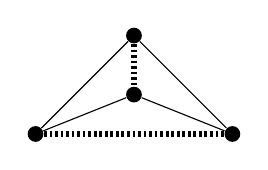
\begin{tikzpicture}
\node at (0,0) [vx](1){};
\node at (0,.75) [vx](0){};
\node at (-1.25,-.5) [vx](2){};
\node at (1.25,-.5) [vx](3){};
\draw (0)--(2)--(1)--(3)--(0);
\draw[grayedge] (0)--(1);
\draw[grayedge] (2)--(3);
\end{tikzpicture} \\
%\includegraphics[scale=.2, trim= 0 0 0 .2cm, clip=true]{figures/paw_4.png}
\hline \\[-2ex]
\ $\indsat{5}{\paw}=1$ & %\includegraphics[scale=.2, trim= 0 0 0 .2cm, clip=true]{figures/paw_5.png}
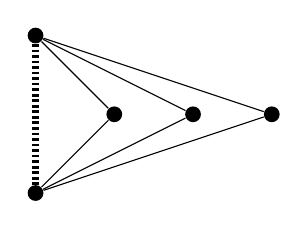
\begin{tikzpicture}
\node at (0,0) [vx](2){};
\node at (1,0) [vx](3){};
\node at (2,0) [vx](4){};
\node at (-1,1) [vx](0){};
\node at (-1,-1)[vx](1){};
\foreach \x in {2,3,4}{\draw (0)--(\x)--(1);}
\draw[grayedge] (0)--(1);
\end{tikzpicture}\\
\hline \\[-2ex]
\ $\indsat{6}{\paw}=1$ & %\includegraphics[scale=.2, trim= 0 0 0 .2cm, clip=true]{figures/paw_6.png}
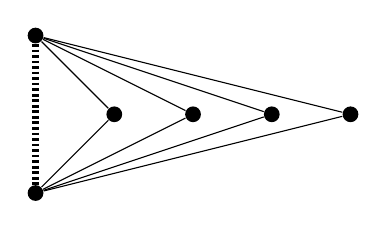
\begin{tikzpicture}
\node at (0,0) [vx](2){};
\node at (1,0) [vx](3){};
\node at (2,0) [vx](4){};
\node at (3,0) [vx](5){};
\node at (-1,1) [vx](0){};
\node at (-1,-1)[vx](1){};
\foreach \x in {2,3,4,5}{\draw (0)--(\x)--(1);}
\draw[grayedge] (0)--(1);
\end{tikzpicture} \\%\bigstrut[t]\\
\end{tabular}
\end{table}



Having established $\indsat{n}{\paw}$ for small values of $n$, we now present our construction.

\begin{cons}\label{cons:paw}
Let $G$ be a graph with at most one trivial component, where each nontrivial component is complete multipartite, each with at least three parts, at most one of which contains only one vertex, and the remainder of which have order at least three.
%Further, every component (except possibly one isolated vertex) has at least three parts, and in any component there is at most one part with only one vertex, and all other parts have at least size three.
\end{cons}


%\iftoggle{sub}{The following is a typical example of a proof that a graph is $H$-induced-saturated.\\}{}

\begin{prop}
The graph $G$ in Construction \ref{cons:paw} is \paw-induced-saturated.
\end{prop}
\begin{proof}
Since \paw is not an induced subgraph of a complete multipartite graph, $G$ contains no induced \paw.
Suppose we add an edge $xy$ such that $x$ and $y$ are in distinct components, say $F_x$ and $F_y$, respectively.  Since at least one of these components, say $F_x$, has at least three parts, $x$ is in some triangle $xab$ in $F_x$.
Because $y$ is in a different component, $y$ is adjacent to $x$ but not $a$ or $b$.
Thus $\{x,y,a,b\}$ induces a \paw.

Suppose we add an edge $xy$ such that $x$ and $y$ are in the same component.
Then in particular, they are in the same part.
This part has at least two vertices, so by construction it has at least three vertices; choose $z$ distinct from $x$ and $y$ from this part, and let $a$ be in another part of the component.
Then $\{x,y,z,a\}$ induces a \paw.

Suppose we delete an edge $xy$.
Then $x$ and $y$ were in different parts of one component, say $F$.
As $F$ is complete multipartite with at least three parts, there exists a vertex $z$ in a third part of that component. Since at most one part has only one vertex, there is a vertex $a$ in the same part as either $x$ or $y$; say $x$. Then $\{x,y,z,a\}$ induces a \paw.
\end{proof}

\begin{cor}\label{indsat_paw}
For $n \ge 7$, $\indsat{n}{\paw}=0$.
\end{cor}


We now show that Construction~\ref{cons:paw} describes all \paw-induced-saturated graphs. %The value of $\sis{n}{\paw}$ follows.

\begin{thm}\label{paw_unique}
A graph is \paw-induced-saturated if and only if it is as described in Construction \ref{cons:paw}.
\end{thm}

To prove this theorem, we begin by making several observations.

\begin{lem}\label{lem:paw_obs}
Let $G$ be a \paw-induced-saturated graph. Then $G$ has the following properties:
\begin{enumerate}[label=(\alph*), ref=\ref{lem:paw_obs}(\alph*)]
%\item\label{K_4-e}  Any edge of $G$ is in an induced copy of $K_4-e$.
\item\label{triangle} Every edge of $G$ is in a triangle.
\item\label{multipartite} The neighborhood of any vertex of $G$ is a complete multipartite graph.
\item\label{book} Given any non-isolated vertex $v \in V(G)$, there exists a (possibly empty) independent set $S=S(v)$ such that for every $x \in N(v)$, $S = N(x) \setminus N[v]$.
\end{enumerate}
\end{lem}
\begin{proof}
%\emph{\ref{K_4-e}.}
%Any edge has the property that its deletion creates an induced copy of the paw.
%Any graph obtained by adding an edge to the paw is isomorphic to $K_4-e$.\\
Lemma~\ref{triangle} holds because deleting any edge in $G$ creates an induced \paw. As a consequence, any vertex has degree either zero or at least two.

Since $G$ does not contain an induced $\paw$, the neighborhood of any vertex cannot contain an induced copy of $K_2 \cup K_1$.
This is equivalent to the neighborhood being a complete multipartite graph. This gives us Lemma~\ref{multipartite}.

To prove Lemma~\ref{book}, suppose there exists $x \in N(v)$ that has a neighbor not in $N[v]$. (If no such $x$ exists, the claim holds with $S = \emptyset$.)
Let $S:=N(x) \setminus N[v]$. If $G[S]$ has an edge $ss'$, then $G[v,x,s,s']$ is a paw. Since $G$ is \paw-induced-saturated, we conclude that $S$ is independent.

By Lemma~\ref{triangle}, there exists $y \in N(v) \cap N(x)$.
If any element $s \in S$ is not adjacent to $y$, then $G[v,x,y,s]$ is a paw with $s$ as the pendant vertex.
Therefore, $S \subseteq N(y)$, but also $N(y)\backslash N[v]\subseteq S$ or else we would have a paw.  Because $N(v)$ is complete multipartite by Lemma~\ref{multipartite}, every vertex in $N(v)\setminus\{x,y\}$ is adjacent to $x$ or $y$.
By symmetry, we conclude that for every $z \in N(v)$, $N(z)\setminus N[v] = S$.
\end{proof}

We proceed to the proof of Theorem~\ref{paw_unique}.
\begin{proof}[Proof of Theorem~\ref{paw_unique}]
Let $G$ be a \paw-induced-saturated graph.  It is clear that $G$ has at most one nontrivial component, since adding an edge between two isolated vertices does not create an induced $\paw$.  We now show that every nontrivial component of $G$ is a complete multipartite graph.
Let $v$ be a non-isolated vertex in $G$ and let $S$ be the set given by Lemma~\ref{book}.
By Lemmas~\ref{multipartite} and \ref{book}, $G[N[v] \cup S]$ is a complete multipartite graph, with $v$ and $S$ sharing a part.
So, we need only show $N[v] \cup S$ is a component of $G$. If not, then there exists some vertex $s \in S$ with a neighbor $t \not\in N[v]\cup S$ since we have included the neighborhood of every $x\in N[v]$ and $S$ is an independent set.
If there exists an edge $xy$ in $G[N(v)]$, then $G[x,y,s,t]$ is a paw, so $N(v)$ is an independent set.
This violates Lemma~\ref{triangle}.

Now, by Lemma~\ref{triangle}, every nontrivial component of $G$ must have at least three parts.
Next, we show that no part in any component of $G$ has order two, and any component has at most two parts of order one. Suppose $x$ and $y$ either make up a part of order two, or are each a part of order one in a component $F$. Then $\{x,y\}$ dominates $F\setminus\{x,y\}$, and so $x$ and $y$ do not appear together in an induced paw, so adding or deleting the edge $xy$ does not create an induced paw. Hence, $G$ being \paw-induced-saturated implies that it can be formed by Construction \ref{cons:paw}.
\end{proof}

%\subsubsection{$\sis{n}{\paw}$, $\sis{n}{P_3+K_1}$}
\begin{cor}\label{sis paw}For $n \geq 7$, let $n\equiv r \mod 7$, where $0 \le r \le 6$. Then
%$15p \leq \sis{n}{\paw} \leq 15p+20$ and
%for $n \geq 35$,
\begin{equation*}\sis{n}{\paw} = \left\{
\begin{array}{cl}\displaystyle\frac{15}{7}n & \mbox{ if } r =0\\
15\lfloor n/7\rfloor+4(r-1) & \mbox{ if } r \neq 0\end{array}
\right..\end{equation*}
% For $n \geq 7$, let $n = 3q+s$ for $0 \le s \le 2$. Then
%\begin{equation*}\sis{n}{P_3+K_1} = \left\{
%\begin{array}{cl}3q & \mbox{ if } s \neq 2\\
%3(q+1) & \mbox{ if } s =2\end{array}
%\right..\end{equation*}
\end{cor}

%\iftoggle{sub}
%{\begin{proof}The bounds follow from Theorem~\ref{paw_unique} and Observation~\ref{thm:complement}. For $n \geq 35$, we can use disjoint copies of $K_{1,3,3}$, $K_{1,3,4}$, and at most one $K_1$ to create a $\paw$-induced-saturated graph, and this minimizes the number of edges in the construction.
%The paw constructions with the fewest number of edges use $p$ nontrivial components, each $K_{1,3,3}$ or $K_{1,3,4}$ if $n$ is large enough.
%Optimal $P_3+K_1$ constructions are the disjoint unions of triangles, with perhaps an isolate or a copy of $K_4$.\end{proof}}

%The uniqueness of the construction for paw-induced-saturated graphs tells us that the number of black edges is minimized when $r\in\{0,1\}$ by taking $p$ components of order seven, and an isolate if possible. When $r\neq0$, we take some components larger, making $p$ nontrivial components as even in size as possible. In the worst case scenario, $n=13$ and we take one component to be $K_{1,3,8}$. This component has $35=15+20$ edges. For $p \geq 5$, we can take every nontrivial component to be $K_{1,3,3}$ or $K_{1,3,4}$; since $e(K_{1,3,4})=15+4$, this gives the desired bound.

%Since $P_3+K_1$ is the complement of the paw, by Observation~\ref{thm:complement} and Theorem~\ref{paw_unique}, the complements of the graphs in Construction~\ref{cons:paw} are the only $P_3+P_1$-induced-saturated graphs. That is, the join of graphs $G_i$, where every $G_i$ (except possibly one trivial $G_i=K_1$) is the disjoint union of at least three cliques, none of which has size 2 and at most one of which has size 1. To minimize the number of edges, we take $G=G_1$ and all cliques have size 3, except one with size 1 if possible, and one with size 4 if necessary. That is, $G$ is the disjoint union of triangles with perhaps an isolated vertex, or an isolated vertex and a copy of $K_4$.
\begin{proof}
Let $G$ be a minimally \paw-induced-saturated graph on $n$ vertices.
From Theorem \ref{paw_unique}, each nontrivial component of $G$ is a complete multipartite graph with at least three parts.
If some nontrivial component $F$ of $G$ has at least three parts, then we form a \paw-induced-saturated graph with strictly fewer edges
 by dropping edges between two of the parts and forming a single larger part.
%  Let $a_1, a_2, \ldots,a_k$ be the size of the parts, in nondecreasing order.
%Then replacing $F$ with $K_{a_1,a_2,\ldots,a_{k-2},a_{k-1}+a_k}$ yields a \paw-induced-saturated graph with fewer edges.
Thus each nontrivial component of $G$ is tripartite.

The number of edges of a complete tripartite graph on $m$ vertices with parts of size $s,t,$ and $m-(s+t)$ is given by $(m-[s+t])(s+t)+st$.
Given the constraints $s\geq1, t\geq3$, and $m\geq t$, we
see that $(m-[s+t])(s+t)$ is minimized when $s+t$ is minimized, i.e. $s+t=4$; also $st$ is minimized when $s+t$ is minimized.
Therefore, $K_{1,3,m-4}$ obtains the smallest number of edges among all complete tripartite graphs on $m$ vertices.

Now, we may assume $G$ has components $F_0,F_1,\ldots,F_i$ with $n(F_0) \in \{0,1\}$
and for $i>0$, $F_i=K_{1,3,n_i-4}$, where $n(F_0)+\sum_{i=1}^kn_i=n$.
Then:
$$e(G) = \sum_{i=1}^k e(F_i)= \sum_{i=1}^k (4n_i-13)=
4n-13k-4v(F_0).$$

Clearly, this is minimized by taking $k$ as big as possible and, subject to this, $n(F_0)=1$.
That is, we take $k=\lfloor n/7 \rfloor$ and
\begin{displaymath}v(F_0)=\left\{\begin{array}{rl}
0 & \mbox{ if 7 divides $n$}\\
1 & \mbox{ else.}
\end{array}
\right.
\end{displaymath}
\end{proof}

\begin{obs}
Given $H$ for which $\sis{n}{H}$ is defined for all sufficiently large $n$,
the function $\sis{n}{H}$ is not necessarily monotone in $n$. In particular, from Corollary~\ref{sis paw} we see for any integer $k \geq 2$,
$\sis{7k}{\paw}<\sis{7k+2}{\paw}<\sis{7k-1}{\paw}$.
This is a similarity between minimal induced saturation and saturation: as noted in~\cite{FFS}, the function $\sat{n}{H}$ is not necessarily monotone in $n$ for fixed $H$.
\end{obs}

%Observe that $K_{1,3,3}$ has fifteen edges,
%  and each additional vertex in a component of a \paw-induced-saturated graph adds at least four edges.
%Thus $G$ must have as many components as possible, and most of these components must be $K_{1,3,3}$.

%Since at most one component of $G$ has fewer than seven vertices, the number of components in $G$ is $\lceil\frac n7 \rceil$.
%Thus each component, except for an isolate when $n$ is not a multiple of seven, contains $K_{1,3,3}$.
%The remaining $r-1$ vertices can be placed in the third part of any of the $K_{1,3,3}$ components.
%Hence the total number of edges in $G$ is $15p$ if $n$ is divisible by seven and $15p+4(r-1)$ otherwise.




%end subsection the paw


%%%%%%%%%%%%%%%%%%%%%%%%%%%%%%%%%%%
%
%        STARS
%
%%%%%%%%%%%%%%%%%%%%%%%%%%%%%%%%%%%

%begin subsection stars
\section{Stars}
 Recall that $K_{1,2} = P_3$, and $\indsat{n}{P_3} = 0$ for $n \ge 3$, as established in \cite{MS}.  In this section we provide a construction extending this result, to show that for fixed $k \ge 2$ and $n$ sufficiently large, $\indsat{n}{K_{1,k+1}}=0$.  Additionally, our construction, together with a simple argument, determines $\sis{n}{K_{1,k+1}}$ within a factor of two.  The case when $k = 2$, which refers to the graph $K_{1,3}$, commonly known as the claw, will be addressed in further detail in Section \ref{sec:claw}.


\begin{cons}\label{cons:stars}
Fix $k \ge 2$ and $n \ge 3^k$.  Let $z,R$ be positive integers such that $n = z3^k + R$ with $0 \le R < 3^k$.  Let $H$ be the graph $K_3^1 \cartprod K_3^2 \cartprod \cdots \cartprod K_3^k$, where $K_3^i$ denotes a single copy of $K_3$.  In other words, $V(H) = \{(\alpha_1,\dots, \alpha_k) : \alpha_i \in [3]\}$, and $(\alpha_1,\dots, \alpha_k)(\beta_1,\dots, \beta_k) \in E(H)$ iff $\sum \{i:\alpha_i\neq\beta_i\} = 1$.  Define $H'$ where $V(H')$ is  the disjoint union of $V(H)$ and $V(K_R)$, and $E(H')$ consists of $E(H),$ $E(K_R)$ and the edges between $H$ and $K_R$ satisfy: for each $v \in V(K_R)$, $v\alpha \in E(H')$ if and only if $\alpha = (\alpha_1,1,1,\dots,1)$, $\alpha_1 \in [3]$.
We now define $G$ to be the disjoint union of $z-1$ copies of $H$ and a single copy of $H'$.
\end{cons}


%%%%%%%%
\begin{comment}
\begin{thm}\label{prop:stars}
For $k \geq 2$ and $n \geq 3^k$, $\indsat{n}{K_{1,k+1}}=0$. % for all $n \geq 3^k$ and $k \geq 1$.
\end{thm}
The basic construction of a $K_{1,k+1}$-induced-saturated graph is simply a Cartesian product of $k$ cliques.
However, this does not suffice to show that $\indsat{n}{K_{1,k+1}}=0$ for all values of $n$.
To obtain a $K_{1,k+1}$-induced-saturated graph on $n$ vertices for any value of $n$, we make use of the fact that for a given $k \geq 2$, any $n \geq 3^k$ can be written as $\prod_{i=1}^k t_i + q$, where $3 \le t_1 \le t_2 \leq \cdots \le t_k$ and $0 \leq q < \prod_{i=2}^k t_i$.
We then take the Cartesian product of the $k$ cliques of orders $t_i$ for $1 \le i \le k$ and add $q$ vertices, in a way that will be specified, to obtain a graph of order $n$.
For a sequence $s=(t_1, \ldots, t_k)$, we will use the notation $K^s$ to represent $K_{t_1}\cartprod \cdots\cartprod K_{t_k}$.



\begin{cons}\label{cons:stars}
Fix $k \geq 2$, and suppose $n=\prod_{i=1}^k t_i + q$, where $3 \le t_1 \le t_2 \leq \cdots \le t_k$ and $0 \leq q < \prod_{i=2}^k t_i$. Let $s_{n,k}=(t_1, \ldots, t_k)$.
If $q=0$, let $G=K^{s_{n,k}}$.
If $q=1$, let $G=K^{s_{n,k}} \cup K_1$.
For $q > 1$, note that $K^{s_{n,k}}$ can be thought of as $t_k$ copies of $K_{t_1} \cartprod \cdots \cartprod K_{t_{k-1}}$.
Let $v_1, \ldots, v_{t_k}$ be the $t_k$ copies of a single vertex of $K^{(t_1, \ldots, t_{k-1})}$ in $K^{s_{n,k}}$, and let $G=K^{s_{n,k}} \cup K_q$ with every vertex in $K_q$ adjacent to each of $v_1, \ldots, v_{t_k}$.
\end{cons}


%Let $s_k:=(t_1,\ldots,t_k)$. We will denote by $K^{s_k}$ the Cartesian product $K_{t_1} \cartprod \cdots \cartprod K_{t_k}$.
%If $t_i \geq 3$ for every $i$, then $K^{s_k}$ is $K_{1,k+1}$-induced-saturated. Moreover,
\begin{lemma}\label{lem:stars1}
%If $k \geq 2$ or $t_1 \geq 4$ for at least one $i$,  then
For $k \geq 2$ and any list $s_k=(t_1, \ldots, t_k)$ with  $3 \le t_1 \le \cdots \le t_k$, the graph $K^{s_k}=K_{t_1} \cartprod \cdots \cartprod K_{t_k}$ is $K_{1, k+1}$-induced-saturated.
Furthermore, for every $v,w \in V(K^{s_k})$, $K^{s_k}$ contains an induced $K_{1,k}$ centered at $v$ that does not contain $w$.
\end{lemma}

\begin{proof}
The proof proceeds by induction on $k$.


For $k=2$, first note that $K_{t_1}\cartprod K_{t_2}$ does not contain an induced $K_{1,3}$. Then we must show that adding or deleting any edge will create an induced $K_{1,3}$. Label the vertices of $K_{t_1}\cartprod K_{t_2}$ with $v_{i,j}$ where $1 \le i \le t_1$ and $1 \le j \le t_2$. (Thus, the set $\{v_{1,j}, v_{2,j}, \ldots, v_{t_1,j}\}$ induces a copy of $K_{t_1}$.)
Let $G'=G-e$, where $e=v_{i,j} v_{i,p}$ for some $p \neq j$, then there is an $\ell$ such that $G'[v_{i,\ell}, v_{i-1,\ell}, v_{i,j},v_{i,p}]$ is isomorphic to $K_{1,3}$, with $v_{i,\ell}$ as the central vertex. If $G'=G-e$ where  $e=v_{i,j}v_{p,j}$, for some $p \neq i$; then there is an $\ell$ such that $G'[v_{\ell,j}, v_{\ell,j-1}, v_{i,j}, v_{p,j}]$ is isomorphic to $K_{1,3}$ with $v_{\ell,j}$ as the central vertex.
If we add an edge, it must be of the form $v_{i,j}v_{\ell,p}$ where $i \neq \ell$ and $j \neq p$.
Then there is an index $m$ such that the graph induced by $\{v_{i,j}, v_{i,p+1}, v_{m, j},v_{\ell,p}\}$ is isomorphic to $K_{1,3}$ (with $v_{i,j}$ as the vertex of degree 3).
Thus, $K^{s_2}$ is $K_{1,3}$-induced-saturated.

For the second part of the claim, choose vertices $v_{i,j}$ and $v_{\ell,p}$ in $V(K^{s_2})$. If $j=p$, then there is an index $\ell'$ such that $G[v_{i,j}, v_{i, j-1},v_{\ell',j}]$ is $K_{1,2}$ with $v_{i,j}$ as the central vertex. If $i=\ell$, then $v_{i,j}$ is the center of a $K_{1,2}$ with $v_{i-1,j}$ and $v_{i,j-1}$ as leaves.
If both $i\neq \ell$ and $j \neq p$, then these vertices are nonadjacent, so $G[v_{i,j}, v_{i-1,j},v_{i,j-1}]$ is a $K_{1,2}$ with center $v_{i,j}$. This establishes the base case.

Now, let $k \geq 3$, and let $s_{k-1}=(t_1,\ldots,t_{k-1})$.
We claim first that $K^{s_k}= K^{s_{k-1}} \cartprod K_{t_{k}}$ contains no induced $K_{1,k+1}$. Notice that $K^{s_k}$ consists of $t_k$ copies of $K^{s_{k-1}}$.
By the induction hypothesis, we know that $K^{s_{k-1}}$ is $K_{1,k}$-induced-saturated, so it does not contain an induced $K_{1,k}$.
Without loss of generality, consider a vertex $v$ in the first copy, say $A$, of $K^{s_{k-1}}$.
The neighborhood of $v$ outside of $A$ induces a clique, so if there were an induced $K_{1,k+1}$ centered at $v$, at least $k$ of its leaves would come from $A$, a contradiction.
This shows that $K^{s_k}$ does not contain an induced $K_{1,k+1}$.
%there is at most one vertex in an induced star centered at $v$ outside its copy of $K^{s_{k-1}}$. By the induction hypothesis, there are at most $k-1$ leaves from inside the copy, so the biggest induced star with $v$ as its center has $k$ leaves.

Suppose we delete an edge $e$ in $K^{s_{k-1}} \cartprod K_{t_k}$. Suppose that the endpoints of $e$ are inside a copy, $B$, of $K^{s_{k-1}}$. By the induction hypothesis, $B$ is $K_{1,k}$-induced-saturated, so there is an induced $K_{1,k}$ inside $B$ that uses both endpoints of $e$.
Including the edge from the center of this $K_{1,k}$ to its clone in another copy of $K^{s_{k-1}}$ yields an induced $K_{1,k+1}$.

If $e$ is an edge between two copies of $K^{s_{k-1}}$, then suppose the endpoints of $e$ are $v_{i,j}$ and $v_{i,\ell}$, where the first coordinate of the index identifies the vertex in $K^{s_{k-1}}$ and the second coordinate indicates which copy of $K^{s_{k-1}}$ the vertices are in. Since $t_k \ge 3$, there is some index $p$ such that $v_{i,p}$ is adjacent to $v_{i,j}$ and $v_{i,\ell}$. By the second half of the claim and the induction hypothesis, the $p$'th copy of $K^{s_{k-1}}$ contains an induced copy of $K_{1,k-1}$ centered at $v_{i,p}$ and avoiding some $v_{i-1,p}$; adding the edges $v_{i,p}v_{i,j}$ and $v_{i,p}v_{i,\ell}$ yields an induced $K_{1,k+1}$.

A similar argument shows that adding an edge to $K^{s_k}$ creates an induced $K_{1,k+1}$, so $K^{s_k}$ is $K_{1,k+1}$-induced-saturated.

To show the second part of the claim,
suppose $v$ and $w$ are two vertices in $K^{s_k}$.
If they are in the same copy of $K^{s_{k-1}}$, then there is an induced $K_{1,k-1}$ centered at $v$ that avoids $w$.
Using any edge from $v$ to its clone in a different copy of $K^{s_{k-1}}$ completes an induced $K_{1,k}$ that avoids $w$.
If $v$ and $w$ are in different copies of $K^{s_{k-1}}$, say $A$ and $B$, respectively, let $w'$ be a copy of $w$ in $A$. By induction, there is an induced $K_{1,k-1}$ in $A$ that is centered at $v$ and avoids $w'$. Using an edge from $v$ to a copy of $v$ in a third copy of $K^{s_{k-1}}$ (distinct from $A$ and $B$) yields an induced $K_{1,k}$ centered at $v$ and avoiding $w$.

\end{proof}
\end{comment}
%%%%%%%%%%%%%%

%\begin{cons}\label{cons:stars2}
%Let $t_i \geq 3$ for every $i$ and let $k \geq 2$. Fix some vertex $v \in$\Kk, and
%create $G$ by adding a clique $Q$ to $K^{s_k}$ such that every vertex in the clique is adjacent to every copy of $v$.
%Then $G$ is $K_{1,k+1}$-induced-saturated.
%\end{cons}


\begin{prop}\label{prop:stars2}
The graphs in Construction \ref{cons:stars} are $K_{1,k+1}$-induced-saturated.
\end{prop}
%\iftoggle{sub}{The proof is straightforward, and so we omit it here.}{
\begin{proof}
Given fixed $n$ and $k$, let $G$ and $R$ be as defined in Construction \ref{cons:stars}.  Let $F$ denote the subgraph of $H'$ isomorphic to $H$.   Suppose to the contrary that $G$ contains an induced $K_{1,k+1}$ with center $x$.  Suppose first that $x$ is in a copy of $H$.  Since $x$ and its neighbors can be represented with $k$-dimensional vectors, by the Pigeonhole Principle, any $k+1$ neighbors of $x$ have two vectors which differ in exactly the same coordinate from each other.  Thus, $x$ cannot have $k+1$ neighbors which form an independent set, and $H$ is $K_{1,k+1}$-free.

If $H'$ contains the induced $K_{1,k+1}$, then $x$ cannot be in the $K_R$ as the neighborhood of $x$ would be a clique.  So $x$ is in $F$.  If this induced $K_{1,k+1}$ contains no vertices from the copy of $K_R$, then the above argument produces  a contradiction.  Thus, this $K_{1,k+1}$ contains a vertex from the copy of $K_R$, and without loss of generality, we may assume that $x$ represented by $(1,1,\dots,1)$ in $F$.  Consequently, our $K_{1,k+1}$ has exactly one vertex in $K_R$, but then contains no vertices of the form $(\alpha_1,1,1,\dots,1)$ other than $x$.  Hence by pigeon hole, $x$ has at most $k-1$ other neighbors in our $K_{1,k+1}$ from $F$, a contradiction.   So $G$ is $K_{1,k+1}$-free.

It is clear that every vertex in a copy of $H$ (or in $F$) is the center of an induced $K_{1,k}$.  Thus, if we add an edge between two components of $G$, one component must be a copy of $H$, and we obtain an induced $K_{1,k+1}$.  Thus, it remains to consider adding an edge within a component.  Note that by the construction of $H'$, the only possible way to add an edge is within $F$, which is isomorphic to $H$.  So, it suffices to consider adding an edge to a copy of $H$.  Suppose we add the edge $uv$.  Without loss of generality, we may assume that $u$ is represented by $(1,1,\dots, 1)$.  Since $u$ and $v$ were not adjacent in $H$, their corresponding vectors must differ in at least two coordinates, say the first and second.  As a consequence, $v$ is adjacent to neither $y$ nor $w$, where $y \in \{(2,1,1,\dots,1), (3,1,1,\dots,1)\}$ and $w \in \{(1,2,1,1,\dots,1), (1,3,1,1,\dots,1)\}$.  Thus, $\{u,v,w,y\}$ is an induced $K_{1,3}$ centered at $u$.  To this set we add vertices $\alpha^3,\alpha^4,\dots, \alpha^k$, where $\alpha^i$ has all coordinates equal to 1 except that the $i$th coordinate is either 2 or 3.  This induces $K_{1,k+1}$.

Lastly, suppose we remove an edge $uv$.  There are three cases to consider.  The first case is if $uv$ is in a copy of $H$ (or in $F$).  Here, we may assume $u = (2,1,1,\dots,1)$ and $v = (3,1,1,\dots,1)$.  The second case is if both $u$ and $v$ are in $K_R$.  The last case is if only, say $v$, is in $K_R$.  Here, we may again assume that $u = (2,1,1,\dots,1)$.  In all three cases, $(1,1,\dots,1)$ together with $u,v,\alpha^2,\dots,\alpha^k$ as defined above, induce a $K_{1,k+1}$.  This completes the lemma.
\end{proof}
%}


%%%%%%%%%%
\begin{comment}
Since $K^{s_{k}}$ does not contain an induced $K_{1,k+1}$, neither does $G$.
Lemma \ref{lem:stars1} shows that if $q=0$, $G$ is $K_{1,k+1}$-induced-saturated.
If $q=1$, then the nontrivial component of $G$ is $K_{1,k+1}$-induced-saturated and removing any edge from $G$ or adding any edge to this component yields an induced $K_{1,k+1}$.
We must only consider adding an edge from the isolated vertex $w$ to the nontrivial component.
Let $v$ be the other endpoint of this edge.
Lemma \ref{lem:stars1} implies that there is an induced $K_{1,k}$ centered at $v$; together with the edge $vw$ we have an induced copy of $K_{1,k+1}$.

If $q > 1$, consider deleting an edge $e$ from $G$. If $e$ is contained in $K^{s_k}$, we have already shown that there is an induced $K_{1,k+1}$ in $G+e$.
Thus, we only consider the cases where $e=uw$ is in $K_q$ or $e$ has one endpoint in $K_q$ and the other in $K^{s_k}$. In the first case, we know that $u$ and $w$ are adjacent to the vertices $v_1, \ldots, v_{t_k}$ in $K^{s_k}$. By Lemma \ref{lem:stars1}, there is an induced $K_{1,k-1}$ in $K^{(t_1, \ldots, t_{k-1})}$ with center $v_1$. Adding the edges $v_1 u$ and $v_1 w$ to this yields an induced $K_{1,k+1}$.

If $u \in K_q$ and $w \in K^{s_k}$, suppose $w$ is in the first copy of $K^{(t_1, \ldots, t_{k-1})}$. Let $w'$ be a copy of $w$ in the second copy of $K^{(t_1, \ldots, t_{k-1})}$. There is an induced $K_{1,k-1}$ centered at $w'$ contained in this second copy of $K^{(t_1, \ldots, t_{k-1})}$. Adding the edges $w'w$ and $w'u$ yields an induced $K_{1,k+1}$.

If we add an edge to $G$, we only need to consider the case where this edge has one endpoint, $w$, in $K^{s_k}$ and the other endpoint, $u$, in $K_q$. There is an induced $K_{1,k}$ centered at $w$ that does not use any of $v_1, \ldots, v_{t_k}$, so adding the edge $wu$ to this gives us an induced $K_{1,k+1}$.


\end{proof}}
\end{comment}
%%%%%%%%%%

\begin{cor}\label{cor:stars}
For fixed $k \ge 2$ and $n \ge 3^k$, $\indsat{n}{K_{1,k+1}} = 0$.
\end{cor}

%Theorem \ref{prop:stars} is an immediate corollary of Lemmas~\ref{lem:stars1} and \ref{lem:stars2}.
%Furthermore, we can show that $\sis{n}{K_{1,k+1}}$ is linear in $n$ for fixed $k \geq 2$ and sufficiently large $n$.

\begin{thm}\label{bound:stars}
For $n \geq 2\cdot 3^k$ and $k \geq 2$, there exist constants $c_1=c_1(k)$ and $c_2 = c_2(k)$ such that $n\frac{k}{2} - c_1 \le \sis{n}{K_{1,k+1}} \leq nk+c_2$.
\end{thm}
\begin{proof}
Given fixed $n$ and $k$, let $G$ and $R$ be as defined in Construction \ref{cons:stars}.

%%%%%%%
\begin{comment}
\begin{proof}
To show the upper bound, let $R$ be the remainder of $n$ upon division by $3^k$. That is, there exists some integer $z$ such that $n=z \cdot 3^k + R$ and $0 \leq R <3^k$. Let $H$ be the Cartesian product of $k$ copies of $K_3$, as in Construction~\ref{cons:stars}. Let $H'$ be the disjoint union of $H$ and $K_R$, %$(R+3^k)$-vertex graph consisting of one copy of $H$ with a clique of size $R$,
with edges between $H$ and $K_R$ as in Construction~\ref{cons:stars}.
We construct an $n$-vertex graph $G$ consisting of the disjoint union of $z -1$ copies of $H$ and one copy of $H'$. We claim $G$ is $K_{1,k+1}$-induced-saturated. Indeed, by Lemmas~\ref{lem:stars1} and \ref{lem:stars2} it suffices to consider adding an edge between one copy of $H$ and one other component. By Lemma~\ref{lem:stars1}, the endpoint in $H$ is the center of a copy of $K_{1,k}$, so the new edge completes an induced $K_{1,k+1}$ subgraph, as desired.
\end{comment}
%%%%%%%%

We  establish $e(G)$ by considering vertex degrees. The component $H'$ has at most $2\cdot 3^k$ vertices, and so (trivially) at most ${2\cdot 3^k \choose 2}$ edges. The remaining vertices, of which there are at most $n-3^k$, all have degree $2k$ for a contribution of at most $(n-3^k)k$ edges. All told, $e(G) \leq nk-k\cdot 3^k + {2\cdot 3^k \choose 2}$.

To show the lower bound, suppose that $G$ is a $K_{1,k+1}$-induced-saturated graph.  Let $S=\{x \in V(G) \colon \deg(x) \le k-1\}$. %\subseteq V(G)$ be the set of vertices such that for all $x \in S$, $\deg(x) \le k - 1$.
We claim that $|S| \le k$.

If $|S| > k$, then there exist $x,y \in S$ such that $xy \notin E(G)$.  Let $G'$ denote $G + xy$.  As $G$ was $K_{1,k+1}$-induced-saturated, $G'$ must contain an induced $K_{1,k+1}$, using the edge $xy$ with either $x$ or $y$ as the center of this $K_{1,k+1}$.  However, as both $x$ and $y$ are adjacent to at most $k - 1$ vertices in $G$, this cannot happen.  So $|S| \le k$, as claimed.

Observe:  $$
|E(G)| \ge  \frac{1}{2}\left(k(n - |S|) + \sum\limits_{x \in S} \deg(x)\right) \ge \frac{nk}{2} - \frac{k^2}{2}.$$

This establishes the lower bound.
\end{proof}

It worth noting that we can extend Construction \ref{cons:stars}, as any graph formed as a Cartesian product of exactly $k$ cliques, each of size at least three, is $K_{1,k+1}$-induced-saturated.


%%%%%%%%%%%%%%%%%%%%%%%%%%%%%%%
%
%            CLAW
%
%%%%%%%%%%%%%%%%%%%%%%%%%%%%%%%


%begin subsection claw
\section{The Claw}\label{sec:claw}
%\todo[inline, color=yellow]{Fact that is used often, but only formally stated in one proof: Let $G$ be a \claw-induced-saturated graph. When edge $xy$ is added, eith $x$ or $y$ is the center of an induced \claw.  When edge $xy$ is removed, both $x$ and $y$ are leaves of an induced \claw.}


For sufficiently large $n$, Theorem \ref{bound:stars} states that the order of magnitude of $\sis{n}{K_{1,k+1}}$ is linear in $n$, and in particular, we know the coefficient within a factor of two.  In this section, we will determine the coefficient of $\sis{n}{K_{1,3}}$, which coincides with the upper bound given in Theorem \ref{bound:stars}.  Additionally, we will provide better constructions than than that in Construction \ref{cons:stars}, which will ultimately determine $\sis{n}{K_{1,3}}$ within an additive constant of four.


%%%%%
\begin{comment}
The star $K_{1,3}$ is also known as the \emph{claw}.  While we have already shown that \claw has induced saturation number zero for sufficiently large $n$, the following constructions will provide graphs that are $K_{1,3}$-induced-saturated with fewer edges than those in Construction \ref{cons:stars} and so will give us a more precise value for $\sis{n}{K_{1,3}}$.
\end{comment}
%%%%%

Values of $\indsat{n}{\claw}$ were determined for $4\leq n \leq 10$ by computer search\footnote{A program was written in C++ and is available at \url{http://www.math.unl.edu/~s-sbehren7/main/Data.html}.} and are listed in \hyperref[tab:claws]{Table~\ref*{tab:claws}}, along with trigraphs that achieve the minimum number of gray edges.
This together with Corollary \ref{cor:stars} determines $\indsat{n}{\claw}$ for all $n$.
We now turn our attention to $\sis{n}{\claw}$.


\begin{table}[htdp]
%\newcolumntype{V}[1]{>{\centering\arraybackslash} m{#1\linewidth} }
\centering
\begin{tabular}{|c||c|}
\hline %\\[-2ex]
%\captionsetup{labelformat=empty, labelsep=none, textformat=empty}
\begin{tabular}{V{.205}|V{.2}}
%\hline \\[-2ex]
$\indsat{4}{\claw}=3$ &
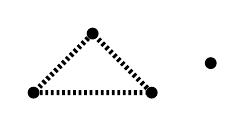
\begin{tikzpicture}[scale=.75]
\node at (1,1) [vx, scale=.75](0){};
\node at (0,0) [vx, scale=.75](1){};
\node at (2,0) [vx, scale=.75](2){};
\node at (3,.5) [vx, scale=.75](3){};
\draw[sgrayedge] (0)--(1)--(2)--(0);
\end{tikzpicture}
\\
\hline \\[-2ex]
$\indsat{5}{\claw}=3$ &
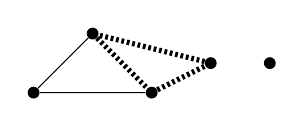
\begin{tikzpicture}[scale=.75]
\node at (1,1) [vx, scale=.75](0){};
\node at (0,0) [vx, scale=.75](1){};
\node at (2,0) [vx, scale=.75](2){};
\node at (3,.5) [vx, scale=.75](3){};
\node at (4,.5)[vx, scale=.75](4){};
\draw[sgrayedge] (0)--(2)--(3)--(0);
\draw (0)--(1)--(2);
\end{tikzpicture}
\\
\hline \\[-2ex]
$\indsat{6}{\claw}=3$ &
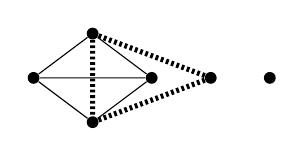
\begin{tikzpicture}[scale=.75]
\node at (0,0) [vx, scale=.75](0){};
\node at (1,.75) [vx, scale=.75](1){};
\node at (1,-.75)[vx, scale=.75](2){};
\node at (2,0)[vx, scale=.75](3){};
\node at (3,0)[vx, scale=.75](4){};
\node at (4,0)[vx, scale=.75](5){};
\draw (0)--(1)--(3)--(2)--(0)--(3);
\draw[sgrayedge] (1)--(2)--(4)--(1);
\end{tikzpicture}
\\
\hline \\[-2ex]
$\indsat{7}{\claw}=2$&
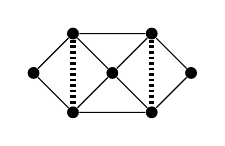
\begin{tikzpicture}
\node at (0,0)[vx, scale=.75](0){};
\node at (1,0)[vx, scale=.75](1){};
\node at (2,0)[vx, scale=.75](2){};
\node at (.5,.5)[vx, scale=.75](3){};
\node at (1.5,.5)[vx, scale=.75](4){};
\node at (.5,-.5)[vx, scale=.75](5){};
\node at (1.5,-.5)[vx, scale=.75](6){};
\draw (0)--(3)--(4)--(2)--(6)--(5)--(0);
\draw (3)--(1)--(5);
\draw (4)--(1)--(6);
\draw[sgrayedge] (3)--(5);
\draw[sgrayedge] (4)--(6);
\end{tikzpicture}\\
\hline \\[-2ex]
$\indsat{8}{\claw}=2$&
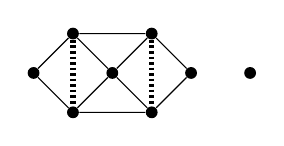
\begin{tikzpicture}
\node at (0,0)[vx, scale=.75](0){};
\node at (1,0)[vx, scale=.75](1){};
\node at (2,0)[vx, scale=.75](2){};
\node at (.5,.5)[vx, scale=.75](3){};
\node at (1.5,.5)[vx, scale=.75](4){};
\node at (.5,-.5)[vx, scale=.75](5){};
\node at (1.5,-.5)[vx, scale=.75](6){};
\draw (0)--(3)--(4)--(2)--(6)--(5)--(0);
\draw (3)--(1)--(5);
\draw (4)--(1)--(6);
\draw[sgrayedge] (3)--(5);
\draw[sgrayedge] (4)--(6);
\node at (2.75,0)[vx, scale=.75](7){};
\end{tikzpicture}
\\
\hline\\[-2ex]
$\indsat{9}{\claw}=0$&
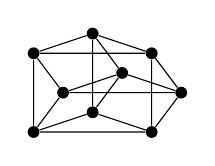
\begin{tikzpicture}[xscale=.75, yscale=.5]
\node at (0,0)[vx, scale=.75](0){};
\node at (1,.5)[vx, scale=.75](1){};
\node at (2,0)[vx, scale=.75](2){};
\node at (.5,1)[vx, scale=.75](3){};
\node at (1.5,1.5)[vx, scale=.75](4){};
\node at (2.5,1)[vx, scale=.75](5){};
\node at (0,2)[vx, scale=.75](6){};
\node at (1,2.5)[vx, scale=.75](7){};
\node at (2,2)[vx, scale=.75](8){};
\draw (0)--(1)--(2)--(0);
\draw (3)--(4)--(5)--(3);
\draw (6)--(7)--(8)--(6);
\draw (0)--(3)--(6)--(0);
\draw (1)--(4)--(7)--(1);
\draw (2)--(5)--(8)--(2);
\end{tikzpicture}
\\
%\hline
\end{tabular}
&\begin{tabular}{V{.22}|V{.19}}
%\hline\\[-2ex]
\multirow{5}{*}{$\indsat{10}{\claw}=0$} &
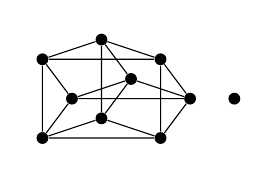
\begin{tikzpicture}[xscale=.75, yscale=.5]
\clip (-.25,-.25) rectangle (3.5, 2.5cm + 2ex);
%\draw[help lines,step=.25cm] (-.25,-.5) grid (4.25, 3.5);
%\draw[help lines,thick,step=1] (0,0) grid (4, 3);
\node at (0,0)[vx, scale=.75](0){};
\node at (1,.5)[vx, scale=.75](1){};
\node at (2,0)[vx, scale=.75](2){};
\node at (.5,1)[vx, scale=.75](3){};
\node at (1.5,1.5)[vx, scale=.75](4){};
\node at (2.5,1)[vx, scale=.75](5){};
\node at (0,2)[vx, scale=.75](6){};
\node at (1,2.5)[vx, scale=.75](7){};
\node at (2,2)[vx, scale=.75](8){};
\node at (3.25,1)[vx, scale=.75](9){};
\draw (0)--(1)--(2)--(0);
\draw (3)--(4)--(5)--(3);
\draw (6)--(7)--(8)--(6);
\draw (0)--(3)--(6)--(0);
\draw (1)--(4)--(7)--(1);
\draw (2)--(5)--(8)--(2);
\end{tikzpicture}
\\ \cline{2-2}\\[-2ex]
&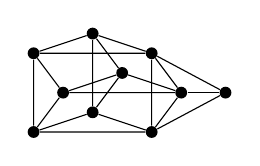
\begin{tikzpicture}[xscale=.75, yscale=.5]
\node at (0,0)[vx, scale=.75](0){};
\node at (1,.5)[vx, scale=.75](1){};
\node at (2,0)[vx, scale=.75](2){};
\node at (.5,1)[vx, scale=.75](3){};
\node at (1.5,1.5)[vx, scale=.75](4){};
\node at (2.5,1)[vx, scale=.75](5){};
\node at (0,2)[vx, scale=.75](6){};
\node at (1,2.5)[vx, scale=.75](7){};
\node at (2,2)[vx, scale=.75](8){};
\node at (3.25,1)[vx, scale=.75](9){};
\draw (0)--(1)--(2)--(0);
\draw (3)--(4)--(5)--(3);
\draw (6)--(7)--(8)--(6);
\draw (0)--(3)--(6)--(0);
\draw (1)--(4)--(7)--(1);
\draw (2)--(5)--(8)--(2);
\foreach \x in {2,5,8} {\draw (9)--(\x);}
\end{tikzpicture}
\\ \cline{2-2}\\[-2ex]
&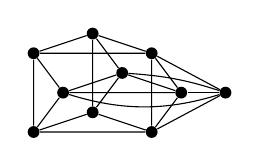
\begin{tikzpicture}[xscale=.75, yscale=.5]
\node at (0,0)[vx, scale=.75](0){};
\node at (1,.5)[vx, scale=.75](1){};
\node at (2,0)[vx, scale=.75](2){};
\node at (.5,1)[vx, scale=.75](3){};
\node at (1.5,1.5)[vx, scale=.75](4){};
\node at (2.5,1)[vx, scale=.75](5){};
\node at (0,2)[vx, scale=.75](6){};
\node at (1,2.5)[vx, scale=.75](7){};
\node at (2,2)[vx, scale=.75](8){};
\node at (3.25,1)[vx, scale=.75](9){};
\draw (0)--(1)--(2)--(0);
\draw (3)--(4)--(5)--(3);
\draw (6)--(7)--(8)--(6);
\draw (0)--(3)--(6)--(0);
\draw (1)--(4)--(7)--(1);
\draw (2)--(5)--(8)--(2);
\foreach \x in {2,5,8} {\draw (9)--(\x);}
\draw (9) to [bend right=10](4);
\draw (9) to [bend left =25](3);
\end{tikzpicture}
\\ \cline{2-2}\\[-2ex]
%\cmidrule(lr){2-3}
&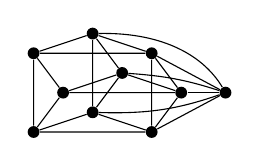
\begin{tikzpicture}[xscale=.75, yscale=.5]
\node at (0,0)[vx, scale=.75](0){};
\node at (1,.5)[vx, scale=.75](1){};
\node at (2,0)[vx, scale=.75](2){};
\node at (.5,1)[vx, scale=.75](3){};
\node at (1.5,1.5)[vx, scale=.75](4){};
\node at (2.5,1)[vx, scale=.75](5){};
\node at (0,2)[vx, scale=.75](6){};
\node at (1,2.5)[vx, scale=.75](7){};
\node at (2,2)[vx, scale=.75](8){};
\node at (3.25,1)[vx, scale=.75](9){};
\draw (0)--(1)--(2)--(0);
\draw (3)--(4)--(5)--(3);
\draw (6)--(7)--(8)--(6);
\draw (0)--(3)--(6)--(0);
\draw (1)--(4)--(7)--(1);
\draw (2)--(5)--(8)--(2);
\foreach \x in {2,5,8} {\draw (9)--(\x);}
\draw (9) to [bend right=10](4);
\draw (9) to [bend left=15](1);
\draw (9) to [bend right=35](7);
\end{tikzpicture}
\\ \cline{2-2}\\[-2ex]
&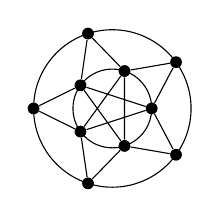
\begin{tikzpicture}[scale=.5]
\foreach \x in {0,1,2,3,4} {\node at (360/5*\x:1cm)[vx, scale=.75](a\x){};}
\foreach \x in {0,1,2,3,4} {\node at (360/5*\x+360/10:2cm)[vx, scale=.75](b\x){};}
\draw (a0)--(b4)--(a4)--(b3)--(a3)--(b2)--(a2)--(b1)--(a1)--(b0)--(a0);
%\draw (b0)--(b1)--(b2)--(b3)--(b4)--(b0);
\draw (0,0) circle (2cm);
%\draw (a0)--(a1)--(a2)--(a3)--(a4)--(a0);
\draw (0,0) circle (1cm);
\draw (a0)--(a2)--(a4)--(a1)--(a3)--(a0);
\end{tikzpicture}
\\
%\hline
\end{tabular}
\tabularnewline\hline
\end{tabular}
\caption{Values of $\indsat{n}{\claw}$ for $4\leq n\leq10$ along with trigraphs realizing those values. All $\claw$-induced-saturated graphs for $n=9$ and $n=10$ are shown.}
\label{tab:claws}
\end{table}


\iftoggle{sub}{
\begin{thm}\label{thm:claw-sis}
For $n \ge 9$, $n \neq 14, 17,$ $2n - 2 \le \sis{n}{K_{1,3}} \le 2n + 2$.
\end{thm}

In order to prove Theorem \ref{thm:claw-sis}, we first prove a series of lemmas.
}{
\begin{thm}\label{thm:claw-sis}
The following bounds hold for $n\geq9$, $n\neq14,17$:
\begin{center}
\begin{tabular}{l c l}
\ $\sis{n}{\claw}=2n$ & if & $n\equiv0\mod3$\\
\ $\sis{n}{\claw}=2n-2$ & if & $n\equiv1\mod3$\\
\ $2n\leq\sis{n}{\claw}\leq2n+2$ & if & $n\equiv2\mod3$
\end{tabular}
\end{center}
\end{thm}

In order to prove Theorem~\ref{thm:claw-sis}, we first prove a series of lemmas that will aid in producing the lower bounds of the statement.
Then we construct families of \claw-induced-saturated graphs that exhibit the upper bounds of Theorem~\ref{thm:claw-sis}.

The following lemma shows that \claw-induced-saturated graphs have few vertices of low degree.
}

\begin{lem}\label{lem:sis_clawdeg}\label{deg2}
Let $G$ be a \claw-induced-saturated graph. Then $G$ has
\begin{enumerate}
\item at most one isolated vertex,
\item no vertices of degree one,
\item at most one vertex of degree two, and
\item at most two vertices of degree three.
\end{enumerate}
%Any graph $G$ that is  \claw-induced-saturated (on $n\geq9$ vertices) does not have any vertices of degree one, has at most one isolated vertex, and has at most one vertex of degree two.
Furthermore, if $G$ has an isolated vertex $v$, then $\delta(G-v)\geq4$.
%If $G$ has an isolated vertex, then $G$ does not have any vertices of degree two or three \textcolor{green}{min deg of G-v is 4};
%otherwise $G$ has at most two vertices of degree three \textcolor{green}{flip}.
\iftoggle{sub}{}{
Additionally, if $G$ has a vertex of degree three, then $G$ does not have a vertex of degree two.
If $G$ has two vertices of degree three or a vertex of degree two, then $G$ has a vertex of degree at least five.
}
\end{lem}
\begin{proof}
%$G$ cannot have two isolated vertices as adding an edge between them does not create a \claw.
Let $G$ be a \claw-induced-saturated graph.  Observe that if we had two isolated vertices, then adding the edge between them would not yield a $K_{1,3}$. Also, any edge of $G$ lies in a triangle, so there are no vertices of degree one.

Suppose that $u$ and $v$ are vertices of degree two. Since every edge lies in a triangle the neighbors of $u$ are adjacent, as are the neighbors of $v$.  Thus, if $u$ and $v$ are not adjacent, adding the edge $uv$ does not create an induced \claw.  If $u$ and $v$ are adjacent, then $N[u] = N[v] = \{u,v,w\}$ for some $w$.  However, removing $uw$ does not create an induced \claw as $v$ would have to have been its center.  So $G$ has at most one vertex of degree two.

To prove $(4),$ suppose $u$ is a vertex of degree three with neighbors $u_1,u_2,u_3$.  Since every edge is in a triangle, we may assume that $u_1u_2, u_2u_3 \in E(G)$.
\textit{Case 1:} $u_1u_3 \notin E(G)$. Then adding $u_1u_3$ creates an induced \claw centered at either $u_1$ or $u_3$; say $u_1$.  Then $u_1$ has two nonadjacent neighbors $x$ and $y$ that are distinct from $u_2$ and $u_3$.  However, $\{u,u_1,x,y\}$ induces a \claw in $G$, a contradiction.  \textit{Case 2:} $u_1u_3 \in E(G)$. In particular, every vertex of degree three in $G$ is contained in a $K_4$.  Let $v$ be another vertex of degree three.  By the above, $N[v]$ induces $K_4$.  If $uv \notin E(G)$, then adding $uv$ does not create an induced \claw.  Thus, $u$ and $v$ are adjacent, and consequently the only vertices of degree three are contained in $N[u]$.

If we remove $uu_1$, then an induced \claw exists, centered at either $u_2$ or $u_3$.   So at least one of them has degree at least four, say $u_3$.  Similarly, removing $uu_3$ creates an induced \claw centered at either $u_1$ or $u_2$ so that at least one of them has degree at least four.  In any case, at most two vertices in $N[u]$, and as a result in $G$, have degree three. Thus, $(4)$ holds.

If $G$ has an isolate, $u$, and another vertex $v$ with $\deg(v) \le 2$, then adding $uv$ cannot create an induced \claw unless $\deg(v) = 2$.  In this case, the neighbors of $v$ cannot be adjacent, however every edge of $G$ must be in a triangle, a contradiction.

%%%%%%%
\begin{comment}
If $uv \in E(G)$, then there exists a vertex $w$ that is the common neighbor of $u$ and $v$, because every edge is in a triangle.
But if we delete $uw$, it does not create a \claw.
Thus $u$ and $v$ are nonadjacent.
Again, because every edge is in a triangle, the two neighbors of $u$ are adjacent and the two neighbors of $v$ are adjacent.
Then adding the edge $uv$ does not create an induced \claw.
Therefore $G$ has at most one vertex of degree two.
If  $G$ has both a vertex $v$ of degree two, and an isolate $s$, then adding the edge $vs$ does not create an induced \claw as the nieghbors of $v$ are adjacent to each other.
Therefore if $G$ has any isolated vertex, it has no vertex of degree two.

Suppose $v\in V(G)$ has degree three.
We will show that $G$ does not have an isolated vertex or a vertex of degree two.
Since every edge is in a triangle, we can say $v$ has neighbors $v_1,v_2,v_3$ with $v_1v_2,v_2v_3 \in E(G)$.
Assume $v_1v_3 \notin E(G)$, so adding the edge $v_1v_3$ creates an induced \claw.
We may assume without loss of generality that $v_1$ is the center of the induced \claw.
Then $v_1$ has two nonadjacent neighbors $x,y$.
Now $\{v,v_1,x,y\}$ induces a \claw, so $v_1v_3 \in E(G)$ and
 the neighborhood of $v$ is a clique.
 In particular, $v$ must be contained in a $K_4$.
This tells us that any $w \in V(G)\setminus N[v]$ has two nonadjacent neighbors from $V[G]\setminus (N[v]\cup w)$ since adding the edge $vw$ must create an induced \claw.
Since every edge is in a triangle, $w$ has at least three neighbors.
As shown above, if $w$ has exactly three neighbors, those neighbors form a clique.
Thus $\deg(w) > 3$ , so there are at most four vertices of degree three, and the vertices of degree three form a clique.
This implies that if $G$ has an isolate, then G has no vertex of degree three, else adding an edge between an isolate and vertex of degree three does not result in an induced \claw.
We also conclude that $G$ does not have a vertex of degree two and a vertex of degree three; such a pair of vertices are nonadjacent, but adding an edge between them does not produce an induced \claw since their neighborhoods are cliques.

By the above argument, a \claw-induced-saturated graph has at most four vertices of degree three; however we claim that such a graph has in fact at most two degree-three vertices.
Let $Q=K_4$ induced by $N[v]$, where $v$ is a degree-three vertex.
Consider deleting an edge $xy$ from $Q$.
Then $x$ and $y$ become leaves in a \claw, so they share a neighbor $r$ that has its own neighbor $s \notin N(x) \cup N(y)$.
If $r \in Q$, then $\deg(r) \geq 4$ because $s \notin Q$.
If $r \notin Q$, then $\deg(x),\deg(y) \geq 4$.
In the latter case, there are at most two vertices of degree three in $G$. In the former case, consider deleting the edge $rx$.
Again, $r$ and $x$ become leaves in a \claw, so there exists a common neighbor $w$ with a private neighbor $z$.
If $w \notin Q$, then $x$ and $r$ have degree at least four, and there are at most two vertices of degree three in $G$.
If $w \in Q$, then $\deg(w)\geq 4$, and $w \neq r$, so  again we have at most two vertices of degree three in $G$.
\end{comment}
%%%%%%%%

\iftoggle{sub}{}{
Suppose $u$ and $v$ are vertices with $\deg(u) = 2$ and $\deg(v) = 3$.  By previous arguments, the neighbors of $u$ form a clique, as do the neighbors of $v$.  Thus, if $uv \notin E(G)$, adding $uv$ does not create an induced $\claw$.  So $uv \in E(G)$, and in particular, $u$ is in the $K_4$ induced by $N[v]$.  However, $\deg(u) = 2$, a contradiction.

Now, suppose $u$ and $v$ are vertices with $\deg(u)=\deg(v)=3$.  By the above, they must be contained in the same $K_4$, so let $u,v,x,y$ denote the vertices of this $K_4$.
If we delete $xy$, then $x$ and $y$ are the leaves of a \claw, but this \claw is not centered at $u$ or $v$, so $x$ and $y$ have a common neighbor $z \not\in \{u,v\}$.
If we delete $xz$, the resulting \claw is centered at a common neighbor of $x$ and $z$.
If that common neighbor is not $y$, then $\deg(x) \geq 5$, and if it is, then $\deg(y) \ge 5$.

Similarly, suppose $\deg(v)=2$, with $N(v)=\{x,y\}$.
Since every edge is in a triangle, $xy \in E(G)$.
If we consider deleting the edge $xy$, we note that the \claw formed does not have center $v$, so $x$ and $y$ share another neighbor $z$, and $z$ has a neighbor $z'$ nonadjacent to both $x$ and $y$.
Consider deleting the edge $vx$. The \claw formed must be centered at $y$, so $y$ has a neighbor nonadjacent to  $v$ or $x$.
Then this neighbor $y'$ is not any of the vertices already named. Similarly, $x$ has a neighbor $x' \not\in \{v,x,y,y',z,z'\}$.
Then $\{x',y'\} \subseteq N(z)$ else $G[x,x',v,z]$ or $G[y,y',v,z]$ is a \claw.
Thus, $\deg(z)\geq 5$.}
\end{proof}

\iftoggle{sub}{}{
\begin{cor}\label{cor:sis_clawmin}
Any graph that is \claw-induced-saturated (on $n \geq 9$ vertices) has at least $2n-2$ edges.
That is, $\sis{n}{\claw} \geq 2n-2$ for $n \geq 9$.
Furthermore, if $G$ is a \claw-induced-saturated graph that does not have an isolated vertex, then $e(G)\geq 2n$.
\end{cor}
\begin{proof}
Apply the degree-sum formula and Lemma~\ref{lem:sis_clawdeg}.
\end{proof}

%%%%%%%%%%%%%%%%%%%%%%%%%%%%%%%%%%%%%%%%%%%%
%%%%%%%%%%%%%%%%%%%%%%%%%%%%%%%%%%%%%%%%%%%%
%\begin{comment}


As indicated in Corollary~\ref{cor:sis_clawmin}, if a graph on $n$ vertices obtaining the minumum number of edges among \claw-induced-saturated graphs exists, then it is four-regular except for an isolated vertex.
We provide the following structural results to show such a graph only exists if $n\equiv1\mod 3$.

\begin{lem}\label{lem:clawnbrs}
Suppose $G$ is a \claw-induced-saturated graph, and for some $v \in V(G)$, every vertex in $N[v]$ has degree precisely 4.
Then $G[N(v)] \in \{2K_2,P_4\}$.
\end{lem}

\begin{proof}

Since we are assuming every vertex in $N[v]$ has degree 4, then we can let $N(v)=\{u,x_1,x_2,x_3\}$. Next, we show that $\Delta(G[N(v)])\leq 2$. Suppose to the contrary that some vertex, say $u\in N(v)$, has three neighbors within $N(v)$; hence, $N(u)\cap N(v)=\{x_1, x_2,x_3\}$. By deleting $ux_1$, we see that $u$ and $x_1$ have a common neighbor besides $v$.
Using the symmetry of $x_1,x_2$, and $x_3$, without loss of generality $x_1x_2,x_2x_3 \in E(G)$.
Now $N(x_2)=\{u,v,x_1,x_3\}$, because $\deg(x_2)=4$.
Consider deleting $ux_1$.
The common neighbors of $u$ and $x_1$ are $v,x_2,$ and maybe $x_3$.
Neither $v$ nor $x_2$ can be the center of a \claw since all of their neighbors are adjacent to $u$ or $x_1$.
Hence $x_3$ must be the center of the induced \claw, so $x_1x_3 \in E(G)$.  But then $N(x_3)=\{v,u,x_1,x_2\}$ so the \claw supposedly centered at $x_3$ has no third leaf.

This shows that  $\Delta(G[N(v)]) \leq 2$.
Because every edge is in a triangle, if $\Delta(G[N(v)]) < 2$, then $G[N(v)]=2K_2$, so suppose $\Delta(G[N(v)])=2$.
Then $G[N(v)]$ is either $C_4$ or $P_4$.

Suppose $x_1x_2x_3x_4=P_4 \subseteq G[N(v)]$.
If $x_1x_4 \not\in E(G)$, then $G[N(v)]=P_4$, so suppose $x_1x_4 \in E(G)$.
Deleting the edge $x_2x_3$ shows that $x_2$ and $x_3$ have a common neighbor $y \in V(G) \setminus N[v]$. Separately, consider deleting $x_3x_4$. The only possible common neighbors of $x_3$ and $x_4$ are $v$ and $y$. Because $x_1x_4 \in E(G),$  $v$ cannot be the center of the \claw created by deleting $x_3x_4$, so the center is $y$. Then the third leaf must be some vertex $y' \not\in N(x_3) \cup N(x_4)$. But we also know that $y' \not\in N(x_2)$, since $\deg(x_2)=4$, so $G[y,y',x_2,x_4]$ is an induced \claw, a contradiction.
\end{proof}


For the remainder of this section, we define $R(G):=\{v\in V(G):G[N(v)]=2K_2\}$ and $B(G):=\{v\in V(G):G[N(v)]=P_4\}$ for any graph $G$.
Hence if $G$ is a four-regular \claw-induced-saturated graph, then $V(G)$ is partitioned into $R(G)$ and $B(G)$.
We will call the vertices in $R(G)$ {\it red vertices} and those in $B(G)$ {\it blue vertices}.


%\begin{rmk}
%We can elaborate on the structure around a blue vertex $v$ in a 4-regular \claw-induced-saturated graph $G$.
%Suppose $x_1x_2x_3x_4=P_4 = G[N(v)]$.
%If we delete $x_2x_3$, the common neighbor at the center of the \claw isn't $v$, because there is no choice for a third leaf.
%Therefore $x_2$ and $x_3$ share some neighbor $y \in V(G)-N[v]$.
%Consider adding the edge $vy$.
%If $v$ is the center of the \claw, then $y$ is not adjacent to $x_1$ or $x_4$. If $y$ is the center of the \claw, then the two other leaves are not adjacent to $v$, so again, $y$ is not adjacent to $x_1,x_4$.
%That means the two as-yet unspecified neighbors of $x_1$ are not in $N[v] + y$.
%This also implies that $y$ is a red vertex: its neighborhood is $2K_2$. Likewise, $x_1$ and $x_2$ are red vertices, while $x_3$ and $x_4$ are blue vertices (Observation \ref{obs:bluetri}).
%\end{rmk}

\begin{lem}\label{lem:bluetri}
If $G$ is a 4-regular \claw-induced-saturated graph, then $B(G)$ induces $kK_3$ for some $k$.
\end{lem}
\begin{proof}
Let $v \in B(G)$ so that $G[N(v)]$ is a path $x_1 x_2 x_3 x_4$.  Since $P_3\subseteq G[\{v,x_1,x_3\}]\subseteq G[N(x_2)]$ and $P_3\subseteq G[\{v,x_2,x_4\}]\subseteq G[N(x_3)]$, Lemma~\ref{lem:clawnbrs} implies that $x_2,x_3\in B(G)$.
Furthermore, as deleting $x_2x_3$ creates an induced \claw, which cannot be centered at $v$, then $x_2$ and $x_3$ share another common neighbor, call it $y$. Since $N(x_2) = \{v,x_1,x_3,y\}$,  $x_1 \in B(G)$ iff $x_1$ and $y$ are neighbors.  So if $x_1y \in E(G)$, we consider adding $vy$ to $G$.  This creates an induced \claw, which must be centered at $y$.  However, since $G$ is 4-regular, $y$ has at most one neighbor outside of $\{x_2,x_3,x_4,v\}$ and cannot be the center of this induced \claw, a contradiction.  Thus, $x_1 \in R(G)$, and by symmetry, $x_4 \in R(G)$.  Repeating the above argument for $x_2$ instead of $v$ shows that $y \in R(G)$.  Hence, $\{x_2,x_3, v\}\subseteq B(G)$ but $N(\{x_2,x_3, v\})=\{x_1,x_4,y\}\subseteq R(G)$ and so $\{x_2,x_3, v\}$ induces a traingle of vertices in $B(G)$.
\end{proof}

An example of a 4-regular \claw-induced-saturated graph, with $R(G),B(G)\neq\emptyset$ is shown in Figure~\ref{fig:claw pretty}.  Observe that $B(G)$ induces $8K_3$, which is in accordance with Lemma~\ref{lem:bluetri}.

\begin{figure}[ht]
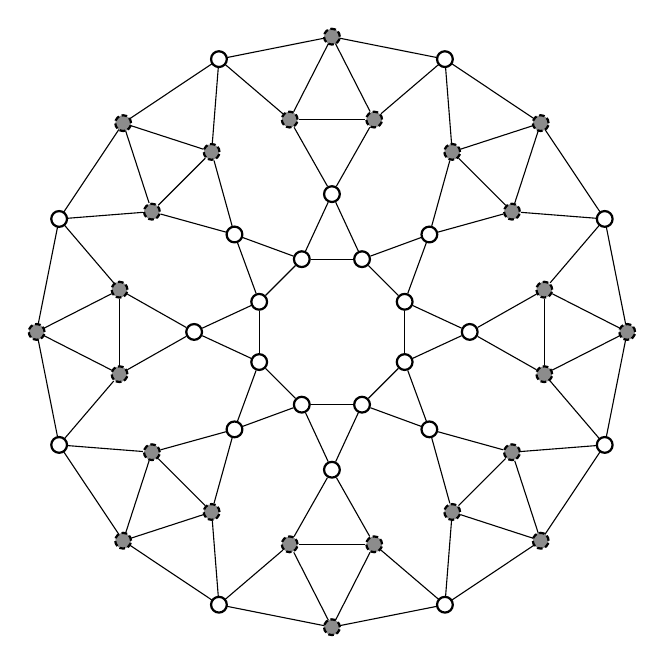
\begin{tikzpicture}
\foreach \x in {0,...,7}
{
\draw[red] (0,0) + (90-360/8*\x:1.75cm) node[whitevx] (A\x){};
\draw[red] (0,0) + (90-360/8*\x+360/16:1cm) node[whitevx] (B\x){};
}
\foreach \x in {0,...,15}
{
\draw[blue] (0,0) + (90-360/16*\x+360/16-360/32:2.75cm) node[grayvx] (C\x) {};
\draw (0,0) + (90-360/16*\x+360/16:3.75cm) node[inner sep=0] (D\x) {};
}
\foreach \x in {0,...,6}
{
\pgfmathparse{int(\x+1)}
\draw (B\x) -- (B\pgfmathresult);
\draw (B\x) -- (A\x) -- (B\pgfmathresult);
}
\draw (B0) -- (A7) -- (B7) -- (B0);
\foreach \x in {0,...,14}
{
\pgfmathparse{int(\x+1)}
\draw (D\x) -- (D\pgfmathresult);
\draw (D\x) -- (C\x) -- (D\pgfmathresult);
}
\draw (D15) -- (C15) -- (D0) -- (D15);
\foreach \x in {0,2,4,6,8,10,12,14}
{
\pgfmathparse{int(\x+1)}
\draw (C\x) -- (C\pgfmathresult);
\draw[red] (D\x)node[whitevx] {};
\draw[blue] (D\pgfmathresult)node[grayvx] {};
}
\foreach \x in {0,...,7}
{
\pgfmathparse{int(2*\x)}
\draw (A\x) -- (C\pgfmathresult);
\pgfmathparse{int(2*\x+1)}
\draw (A\x) -- (C\pgfmathresult);
}
\end{tikzpicture}\caption{A 4-regular \claw-induced-saturated graph. Vertices in $R(G)$ are white, and vertices in $B(G)$ are gray.}\label{fig:claw pretty}
\end{figure}


\begin{lem}\label{lem:adj}
Let $G$ be a 4-regular \claw-induced-saturated graph.
Every edge of $G$ is in either one or two triangles, and there are $|B(G)|$ edges that are in two triangles.
\end{lem}
\begin{proof}
Recall that every edge in a \claw-induced-saturated graph is in at least one triangle.
Suppose there exists $xy \in E(G)$ where $x$ and $y$ have three common neighbors $u,v,w$.
Then $G[N(x)]$ cannot be in $\{2K_2, P_4\}$, which contradicts Lemma \ref{lem:clawnbrs}. Hence, each edge is in at most two triangles.

Let $b$ be the number of edges that are in two triangles.
Label edge $xy$ with vertex $z$ if $xyz$ is a triangle, and allow for multiple labels.
Thus $b$ edges have two labels and hence
$$|E(G)|+b=\sum_{z\in V(G)}|\{e\in E(G): e \text{~has~label~} z\}|.$$
Since each red vertex gives its label to two triangles and each blue vertex gives its label to three triangles, we have $\sum_{z\in V(G)}|\{e\in E(G): e \text{~has~label~} z\}|=2|R(G)|+3|B(G)|$. Thus, since $G$ is 4-regular,

\begin{align*}
2n+b&=|E(G)|+b\\
&= \sum_{z\in V(G)}|\{e\in E(G): e \text{~has~label~} z\}|\\
&=2|R(G)|+3|B(G)|\\
&= 2(n-|B(G)|)+3|B(G)|\\
&=2n+|B(G)|\\
\end{align*}

Therefore, there are precisely $|B(G)|$ edges that are in two triangles.
\end{proof}

%A more careful analysis of the edges in two triangles reveals that for every blue vertex v whose neighborhood is a $P_4=u_1u_2u_3u_4$, the edge $u_2u_3$ is in two triangles.

\begin{prop}\label{3|n}
If $G$ is a 4-regular, \claw-induced-saturated graph on $n$ vertices, then $n\equiv0\mod3$.
\end{prop}
\begin{proof}
Let $b=|B(G)|$.
By Lemma~\ref{lem:bluetri}, 3 divides $b$.
By Lemma~\ref{lem:adj}, $2n-b$ edges are in precisely one triangle, and $b$ edges are in precisely two triangles.
If $t$ is the number of triangles in $G$, then
$3t=(2n-b)+(2b)=2n+b$. Since 3 divides $b$, we know 3 divides $2n$, and so 3 divides $n$.
\end{proof}


The previous lemmas will be used in the proof of Theorem~\ref{thm:claw-sis} to obtain a lower bound $\sis{n}{\claw}\geq2n-1$ for $n \equiv 0 \mod 3$.
The next two propositions show that certain degree sequences do not have a \claw-induced-saturated realization.
This allows us to increase the lower bound of $\sis{n}{\claw}$ for certain values of $n$.

\begin{prop}\label{554}If $G$ is a \claw-induced-saturated graph, then the degree sequence of $G$ is not $(5,5,4,\ldots,4)$.
\end{prop}
\begin{proof}
Suppose $G$ is a counterexample to the claim, and let $v$ be a vertex of degree 5.

\begin{case} $\Delta(G[N(v)])=4$.\end{case}
That is, $v$ has a neighbor $u$ such that $X:=N(u)\cap N(v)$is a set of order 4.
If we delete $vx'$ for some $x' \in X$, then the resulting \claw is not centered at $u$ since the neighbors of $u$ are adjacent to $v$.
Thus $x'$ and $v$ share a neighbor $x\in X$ and there is some $\in N(x)\setminus[N(x')\cup N(v)]$.
Now $N(x)=\{u,v,x',y\}$ and $uy,vy,x'y\notin E(G)$, so the edge $xy$ is in no triangle, a contradiction.

\begin{case}\label{Case3} $\Delta(G[N(v)])=3$. \end{case}
That is, there exist $u \in N(v), w\notin N[u],$ and $X\subseteq N(u)$ with $|X|=3$ so that  $N(v)=\{u,w\} \cup X$. Since deleting the edge $vw$ creates a \claw,
there exist vertices $x'$ and $y$ such that $x'$ is a common neighbor of $v$ and $w$, $y$ is adjacent to $x'$, and $y$ is not adjacent to $w$ nor $v$. Note $x' \in X$ and $y \notin N[v]$.
Then to prevent a \claw in $G$ with center $x'$ and leaves $u,w,y$, we have $uy \in E(G)$. Then, $u,v$ are the vertices of degree 5 and all other vertices have degree 4 so that $N(x')=\{u,v,y,w\}$. Since $u$ is not the center of a \claw, and $x'$ has no neighbors in $X$, the vertices of $X\setminus\{x\}$ (call them $a$ and $b$) are adjacent.

Note that $u$ was chosen as an arbitrary vertex of $N(v)$ with three neighbors in $N(v)$, and we showed $\deg(u)=5$.

Now, $\deg(a)=\deg(b)=4$ and each of $a$ and $b$ currently has two neighbors in $N(v)$. If $a$ (or $b$) were adjacent to $w$, then the argument previously applied to $u$ would guarantee that $\deg(a)=5$ (or $\deg(b)=5$), thus giving us at least three vertices of degree 5. Therefore $a$ and $b$ each have a neighbor outside of $N[v]$; due to the necessity that every edge be in a triangle, they share this neighbor, which we shall name $z$.
It is possible that $z=y$.  Suppose $z\neq y$, then deleting $az$ should create an induced \claw centered at at common neighbor of $a$ and $z$.  However, the only option is $b$, which is not the center of such a \claw, a contradiction.  So suppose $z = y$, then $\deg_{N(u)}(a)=3$. By the previous argument with $u$, we must have $\deg_G(a)=5$, a contradiction.

\begin{case} $\Delta(G[N(v)])\leq 2$. \end{case}
$N(v)$ has no independent set of size three, lest it be the center of a \claw.
Then $G[N(v)] \in \{K_2 + K_3,C_5\}$.

Suppose first $G[N(v)]=K_2 + K_3$, with $\{x_1,x_2,x_3\}$ inducing $K_3$.
We may suppose $\deg(x_1)=\deg(x_2)=4$ since at most one of the vertices in the copy of $K_3$ may have degree 5. So each of $x_1$ and $x_2$ have a neighbor outside of $N[v]$, say $y$ and $z$, respectively.  If $y \neq z$, then since every edge is contained in a triangle, $x_3$ is adjacent to both $y$ and $z$.  However, this implies that $\deg(z) = 5$ and $\Delta(G[N(z)]) \ge 3$, as evidenced by $x_1$.  This puts us in Case \ref{Case3}.

So $y = z$, and consequently, $N[x_1] = N[x_2]$.   The only common neighbors of $x_1$ and $y$ are $x_2$ and possibly $x_3$. If $x_3\notin N(x)\cap N(y)$, removing $x_1y$ should create an induced \claw centered at $x_2$, but it does not.  Thus, removing $x_1y$ creates an induced \claw centered at $x_3$, which implies that $x_3$ is adjacent to $y$, as well as another vertex $y'$ not in $N[v] \cup \{y\}$.  However, this implies that $\deg(x_3)=5$, and $\Delta(G[N(x_3)]) \geq 3$, as evidenced by $x_1$.  This also puts us in Case \ref{Case3}.


Suppose now $G[N(v)]=C_5$ with cycle $x_1x_2x_3x_4x_5$.
We may assume that $x_1,x_2,x_3,$ and $x_4$ all have degree 4.
The only common neighbors of $v$ and $x_2$ are $x_1$ and $x_3$.  When removing $vx_2$ we obtain an induced claw centered at either $x_1$ or $x_3$.  Without loss of generality, assume it is $x_3$.  Since $x_4$ is not a leaf of a \claw that  features $v$ as a leaf, $x_3$ has a neighbor $y \not\in N(v) \cup N(x_2)$. Since $G[x_3,x_2,x_4,y]$ cannot be a \claw, we must have $yx_4 \in E(G)$. Similarly, if we delete $vx_3$, the candidates for center of the ensuing \claw are $x_2$ and $x_4$; we know the neighborhood of $x_4$, and so see that $x_2$ is the center. Then there exists $y' \in N(x_2)$ such that $y' \not\in N(v) \cup N(x_3)$, and as before $y'x_1 \in E(G)$. Now we know the neighborhoods of $x_1,x_2,x_3$, and $x_4$. If we add the edge $x_1x_4$, we find that no \claw is formed, a contradiction.
\end{proof}

\begin{prop}\label{644}
Let $G$ be a \claw-induced-saturated graph. Then for any $n \geq 7$, the degree sequence of $G$ is \emph{not} $(6,4,\ldots,4)$.
\end{prop}
%actually holds for any (a4444) if a \geq 6
\begin{proof}
Suppose $G$ is a counterexample to this claim. Let $v$ have degree six, and let $F=G[N(v)]$, so $|F|=6$, $\Delta(F) \leq 3$, and $\alpha(F) \leq 2$ else $v$ is the center of a \claw. In fact $\alpha(F)=2$ in order for the vertices of $N(v)$ to have degree four in $G$.
If $\delta(F)=3$, then $N[v]$ is a component of $G$, and this component is \claw-induced-saturated.
However, from the computer search, with results listed in Table~\ref*{tab:claws}, we know that there is no nontrivial \claw-induced-saturated graph on fewer than nine vertices.
Therefore $\delta(F) \leq 2$.
Indeed, we claim $\delta(F)=2$.
If $\delta(F) \leq 1$, let $u$ be a vertex with minimum $F$-degree (i.e. $\deg_F(u)$ is minimum), and let $T=F\setminus N[u]$.
Then $T$ is a clique, else two nonadjacent vertices in $T$ together with $u$ and $v$ form a \claw.
Hence $|T|=4$ and the vertices of $T$ have no neighbors outside of $N[v]$ in $G$.
Now, deleting the edge between $v$ and any vertex of $T$ does not create an induced \claw, so $\delta(F)=2$.

Let $u$ be a vertex in $F$ with $\deg_F(u)=2$, and let $T=F\setminus N[u]$.
As before, $T$ is a clique, specifically a triangle.   Let $N_F(u) = \{u', u''\}$.
Since $\deg_F(u)=2$, $u$ has one neighbor $w$ outside of $N[v]$; since every edge is in a triangle, we may assume that $w$ is adjacent to $u'$.  Now, the only common neighbors of $v$ and $u$ are in $N_F(u)$.
Since $\delta(F)=2$, $u'$ must have another neighbor in $F$ other than $u$.  Thus, the only neighbor of $u'$ not in $N[v]$ is $w$, and if we delete $vu$, the resulting induced \claw cannot be centered at $u'$.  So it must be centered at $u''$, which in turn has a neighbor $w''$ outside of $N[v] \cup \{w\}$.  Since $u''w''$ is in a triangle and $\delta(F) = 2$, $u''$ and $w''$ share a neighbor $t''$ in $F$.
Since $\delta(F) = 2$, no vertex in $F$ has two neighbors outside $N[v]$.  So $t'' \neq u'$, and hence $t'' \in T$.
But now $\deg(t'') \geq 5$, a contradiction.
\end{proof}
%\end{comment}
%%%%%%%%%%%%%%%%%%%%%%%%%%%%%%%%%%%%%%%%%%%%%%%
%%%%%%%%%%%%%%%%%%%%%%%%%%%%%%%%%%%%%%%%%%%%%%%


Finally, we construct graphs which we use to find an upper bound for $\sis{n}{\claw}$.
}
%%%%%%%%%%%%%%%%%%%%%%%%%%%%%%%%
%%%%%%%%%%%%%%%%%%%%%%%%%%%%%%%

\begin{lemma}\label{suff_claw}
%Suppose $G$ is a graph such that every edge is in a triangle, the neighborhood of every vertex induces $2K_2$, and $G$ does not contain $K_4-e$\todo{Isn't this implied by the first assumption?}.
If $G$ is a graph where the neighborhood of every vertex induces $2K_2$, then $G$ is \claw-induced-saturated.
\end{lemma}
\begin{proof}
%Since $R(G)$=$V(G)$, then for any vertex $v\in V(G)$, $G[N(v)]\neq P_3$.
%Thus $G$ does not contain $K_4-e$.
Since no vertex has three independent neighbors, $G$ contains no induced \claw.   Suppose we delete an edge $xy$.
Since every edge is in a triangle, say $xyz$, deleting $xy$ leaves $z$ as the center of a \claw with leaves $x$, $y$, and any other neighbor of $z$.
If we add an edge between two vertices with no common neighbors, then we take the new edge together with two nonadjacent neighbors of one of the vertices and find a \claw.
Therefore it suffices to consider adding an edge $xy$, where $x$ and $y$ share a neighbor.
Let $N(x)=\{u_1,u_2,v_1,v_2\}$ with $u_1u_2,v_1v_2 \in E(G)$, and suppose $u_1 \in N(y)$.
Then $u_2 \notin N(y)$ otherwise $N(u_2)$ would contain a $P_3$ and not be $2K_2$.  Similarly, both $v_1$ and $v_2$ cannot be in $N(y)$.  So we may assume $v_2 \notin N(y)$.  Then upon adding $xy$, $\{x,y,u_2,v_2\}$ induces a \claw.
\end{proof}

\begin{lemma}
Let $G$ be a graph with at most one isolated vertex, where each nontrivial  component is one of the graphs in Figure~\ref{fig:claw-i-s}.  Then $G$ is \claw-induced-saturated.
\end{lemma}

\begin{figure}
\centering
\subcaptionbox{$H=K_3\cartprod K_3$, 9 vertices\label{k3xk3}}[.4\linewidth]{
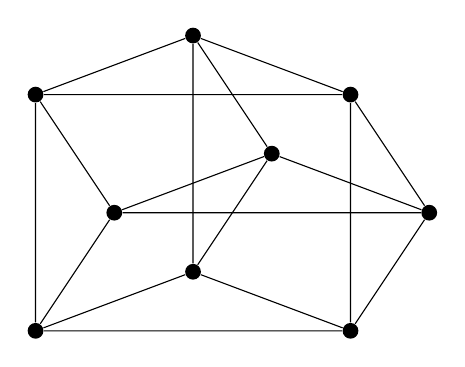
\begin{tikzpicture}[xscale=2, yscale=1.5]
\node at (0,0)[vx](0){};
\node at (1,.5)[vx](1){};
\node at (2,0)[vx](2){};
\node at (.5,1)[vx](3){};
\node at (1.5,1.5)[vx](4){};
\node at (2.5,1)[vx](5){};
\node at (0,2)[vx](6){};
\node at (1,2.5)[vx](7){};
\node at (2,2)[vx](8){};
\draw (0)--(1)--(2)--(0);
\draw (3)--(4)--(5)--(3);
\draw (6)--(7)--(8)--(6);
\draw (0)--(3)--(6)--(0);
\draw (1)--(4)--(7)--(1);
\draw (2)--(5)--(8)--(2);
\end{tikzpicture}
}\hspace{1cm}
\subcaptionbox{Graph $J$ on 11 vertices\label{11vtcs}}[.4\linewidth]{
%\includegraphics[scale=.5]{figures/claw_11}
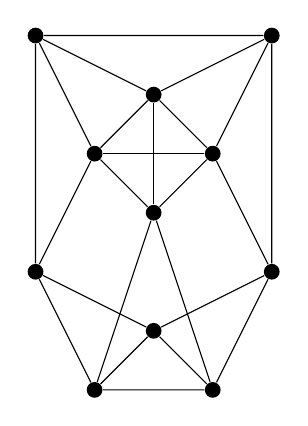
\begin{tikzpicture}[scale=.75]
\draw (0,0) node[vx](b1) {};
\draw (2,0) node[vx](b2) {};
\draw (1,1) node[vx](b3) {};
\draw (b1)--(b2)--(b3)--(b1);
\draw (-1,2) node[vx](r1) {};
\draw (3,2) node[vx](r2) {};
\draw (b1)--(r1)--(b3)--(r2)--(b2);
\draw (1,3) node[vx](g1) {};
\draw (0,4) node[vx](g2) {};
\draw (2,4) node[vx](g3) {};
\draw (1,5) node[vx](g4) {};
\foreach \x in {1,...,4}
	{\foreach \y in {1,...,\x}
		\draw (g\x)--(g\y);}
\draw (-1,6) node[vx](b4) {};
\draw (3,6) node[vx](b5) {};
\draw (g2)--(b4)--(g4)--(b5)--(g3);
\draw (g2)--(r1)--(b4)--(b5)--(r2)--(g3);
\draw (b1)--(g1)--(b2);
\end{tikzpicture}
}
\subcaptionbox{Graph $K$ on 12 vertices\label{12vtcs}}[.4\linewidth]{
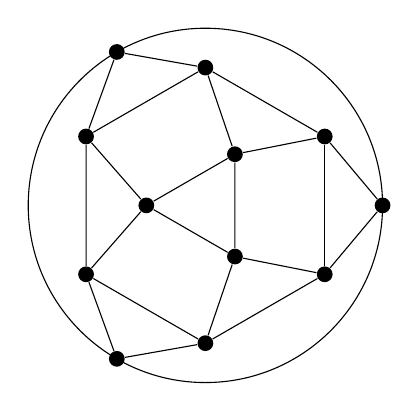
\begin{tikzpicture}[scale=0.25]
\draw (0,0) circle (9cm);
\foreach \x in {1,...,6}
{
\draw (150-60*\x:7cm) node[vx] (A\x) {};
}
\foreach \x in {1,3,5}
{
\draw (120-60*\x:3cm) node[vx] (B\x) {};
}
\foreach \x in {2,4,6}
{
\draw (120-60*\x:9cm) node[vx] (C\x) {};
\pgfmathparse{int(\x-1)}
\draw (C\x) -- (A\x) -- (A\pgfmathresult);
}
\draw (A1) -- (C6);
\draw (A3) -- (C2);
\draw (A5) -- (C4);
\foreach \x in {1,3,5}
{
\pgfmathparse{int(\x+1)}
\draw (B\x) -- (A\x);
\draw (A\pgfmathresult) -- (B\x);
}
\draw (B1) -- (B3) -- (B5) -- (B1);
\draw (A1) -- (A6);
\draw (A2) -- (A3);
\draw (A4) -- (A5);
\end{tikzpicture}
}
\subcaptionbox{Graph $L$ on 15 vertices\label{15vtcs}}[.4\linewidth]{
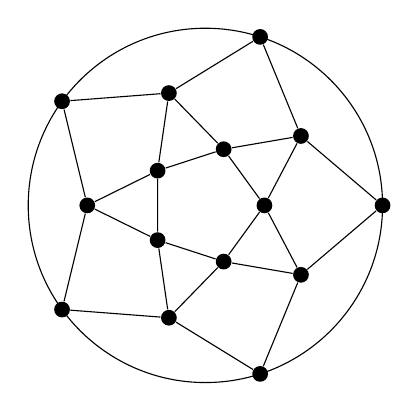
\begin{tikzpicture}
\draw (0,0) circle (2.25cm);
\foreach \x in {1,2,3,4,5}{\draw  (360/5*\x:0.75cm)  node[vx](a\x){};}
\foreach \x in {1,2,3,4,5}{\draw  (36+360/5*\x:1.5cm)  node[vx](b\x){};}
\draw (a1)--(a2)--(a3)--(a4)--(a5)--(a1);
\foreach \x in {1,2,3,4,5}{\draw  (360/5*\x:2.25cm)  node[vx](c\x){};}
\draw (a1)--(b1)--(a2)--(b2)--(a3)--(b3)--(a4)--(b4)--(a5)--(b5)--(a1);
\draw (c1)--(b1)--(c2)--(b2)--(c3)--(b3)--(c4)--(b4)--(c5)--(b5)--(c1);
\end{tikzpicture}
}
\caption{These graphs are \claw-induced-saturated.}\label{fig:claw-i-s}
% For each graph $G$, white vertices belong to $R(G)$ and gray vertices belong to $B(G)$.
\end{figure}

\begin{proof}
By inspection, the graph in Figure ~\ref{11vtcs} is \claw-induced-saturated, and since the graphs in Figures \ref{k3xk3}, \ref{12vtcs}, and \ref{15vtcs} have the property that the neighborhood of every vertex induces $2K_2$, they are \claw-induced-saturated by Lemma~\ref{suff_claw}.
%\iftoggle{sub}{Straightforward case analysis shows that the graph in Figure~\ref{11vtcs} is \claw-induced-saturated.}
%%%%%%%%
%{ Next we show that the graph $J$ in Figure~\ref{11vtcs} is \claw-induced-saturated.
%%%%%%%
\begin{comment}
Next we show that the graph $J$ in Figure \ref{11vtcs} is \claw-induced-saturated.

No induced \claw is centered at a white or gray vertex, because their neighborhoods prohibit it. The graph induced by the neighborhood of every green vertex contains $K_3 + K_2$, so also no induced \claw is centered at a black vertex, so the graph $J$ in Figure \ref{11vtcs} has no induced \claw subgraph.

Every vertex of $J$ is the center of an induced $K_{1,2}$. So, when we consider adding edges, we need only consider adding the edge $xy$ where $x$ and $y$ have a common neighbor.
%(This includes adding edges to other components.)
If $x$ and $y$ share only one neighbor, either can be the center of the induced \claw formed, since there are two nonadjacent neighbors besides the shared neighbor.
Suppose $x$ and $y$ share two neighbors.
The only such cases are when $x$ and $y$ are a black vertex and a gray vertex, or a white vertex with another vertex.
In the case that some vertex is white, a \claw is found centered at the other vertex.
Suppose $x$ is black and $y$ is gray.
The shared neighbors are at the center of the $P_4$ in $N(y)$, so a \claw exists centered at $y$ with leaves $x$ and $N(y)-N(x)$.

Suppose we delete an edge from $J$. If both endpoints of the edge are in the neighborhood of a white vertex or gray vertex, and in the latter case are not the middle edge of the $P_4$, then that vertex is the center of an induced \claw. If both endpoints are in the neighborhood of a black vertex, some black vertex is the center of the induced \claw created.
 Every edge falls into at least one of these categories. We conclude $J$ is \claw-induced-saturated.
%}
\end{comment}
 %%%%%%%%%%%%%%

Now let $G$ be a graph with at most one isolated vertex and each of the remaining components are one of the graphs from Figure~\ref{fig:claw-i-s}.
Since each nontrivial component of $G$ is \claw-induced-saturated, we only need to consider adding an edge $xy$ between components.    When we add the edge $xy$, at least one of $x$ and $y$ must be in a nontrivial component, say $x$.  By inspection we see every vertex in every graph of Figure \ref{fig:claw-i-s} has two nonadjacent neighbors, and in particular, this holds for $x$.  Thus, $x$ together with these two neighbors  and $y$ induce a \claw.  Therefore, $G$ is \claw-induced-saturated.
\end{proof}


%%%%%%%%%%%%%%%%%%%%%%%%%%%%%%%%%%%%%%%%%%%%%%%%%%%%%%%%%%%%%

We now can prove Theorem \ref{thm:claw-sis}.

\begin{proof}[Proof of Theorem \ref{thm:claw-sis}]
\iftoggle{sub}{
Lemma \ref{lem:sis_clawdeg} together with the degree-sum formula gives us the lower bound of $2n - 2$.  To obtain the upper bound, we contruct graphs using $H, J, K$, and $L$ from Figure \ref{fig:claw-i-s}.  These constructions will be based on the residue class of $n$ modulo 3.

\begin{case}\label{0mod3}
$n \equiv 0 \mod 3$, $n \geq 9$
\end{case}
Use $\lfloor n/9 \rfloor-1$ copies of $H$, together with one copy of $H$, $K$, or $L$, for a graph with $2n$ edges.

\begin{case}
$n \equiv 1 \mod 3$, $n \geq 10$
\end{case}
Use an isolated vertex with a graph from Case~\ref{0mod3} for a graph with $2n-2$ edges.
\begin{case}
$n \equiv 2 \mod 3$, $n\geq20$ or $n=11$.
\end{case}
If $n=11$, the graph $J$ suffices. If $n > 11$, then take $J$ and a construction from Case~\ref{0mod3}. This achieves $2n+2$ edges.
}
{
We exhibit graphs with the desired number of edges to prove the upper bounds.

\begin{case}\label{0mod3}
$n \equiv 0 \mod 3$, $n \geq 9$
\end{case}
Use $\lfloor n/9 \rfloor-1$ copies of $H$, together with one copy of $H$, $K$, or $L$, for a graph with $2n$ edges.
Alternatively, we could generalize $L$ for $n\geq 15$ by having $n/3$ vertices in the outer cycle, $n/3$ vertices in the inner cycle, and $n/3$ vertices between the two cycles.
\begin{case}
$n \equiv 1 \mod 3$, $n \geq 10$
\end{case}
Use an isolated vertex with a graph from Case~\ref{0mod3} for a graph with $2n-2$ edges.
\begin{case}
$n \equiv 2 \mod 3$, $n\geq20$ or $n=11$.
\end{case}
If $n=11$, the graph $J$ suffices. If $n \geq 20$, then take $J$ and a construction from Case~\ref{0mod3}. This achieves $2n+2$ edges.

For the lower bound, let $G$ be any \claw-induced-saturated graph.
Corollary \ref{cor:sis_clawmin} gives us a general lower bound of $2n-2$.
Suppose $G$ has no isolated vertex. Then by Corollary~\ref{cor:sis_clawmin}, $e(G) \geq 2n$, as desired. Suppose then that $G$ does have an isolated vertex, and $n \not\equiv 1 \mod 3$. Then $(n-1) \not\equiv 0 \mod 3$, so by Lemmas~\ref{lem:sis_clawdeg} and \ref{3|n}, the minimum degree of the non-isolated vertices is at least 4, and $\Delta(G) \geq 5$. Then
$e(G) \geq \big\lceil\frac{4(n-1)+1}{2}\big\rceil=2n-1$, with equality only if the degree sequence of $G$ is $(5,5,4,\ldots,4,0)$ or $(6,4,\ldots,4,0)$. Since the graph obtained by deleting the isolate is \claw-induced-saturated, by Propositions~\ref{554} and $\ref{644}$, $e(G) \geq 2n$.}
\end{proof}

\iftoggle{sub}{
It is worth noting that for $n \equiv 1 \mod 3$, $n \ge 10$, $\sis{n}{K_{1,3}} = 2n - 2$.  Additionally, a detailed case analysis of degree sequences of $K_{1,3}$-induced-saturated graphs  shows that $\sis{n}{K_{1,3}} \ge  2n$ for $n \not\equiv 1 \mod 3$.  In particular, this implies $\sis{n}{K_{1,3}} = 2n$ for $n \equiv 0 \mod 3$, $n \ge 9$, and $2n \le \sis{n}{K_{1,3}} \le 2n + 2$ for $n \equiv 2 \mod 3$, $n \ge 20$.
}{}

%end \claw subsubsection


%%%%%%%%%%%%%%%%%%%%%%%%%%
%
%         C4 AND MATCHINGS
%
%%%%%%%%%%%%%%%%%%%%%%%%%%

\section{$C_4$ and its complement}\label{sec:small cycles}

In this section we show that the induced saturation number of $C_4$ is zero for sufficiently large $n$, and we compute some bounds on $\sis{n}{C_4}$. Additionally, using Observation \ref{thm:complement} and the fact that $\overline{C_4}=2K_2$, we use $C_4$-induced-saturated graphs to obtain results for matchings.

%We begin with a general construction.

\begin{cons}\label{gen gen icos}
For $j \geq 5$ and $k \geq 2$, let $I_j^k$ be the graph that combines $k$ copies of a wheel with $j$ spokes.  Label the copies $W^1,\ldots,W^k$, and label the vertices of $W^i$ so that its center is $w_0^i$, and the outer cycle of $W^i$ is $w_1^i,\ldots,w_j^i$. For $1\leq i<i^*$,  add the edges $w^i_\ell w^{i^*}_\ell$ and $w^i_\ell w^{i^*}_{\ell+1}$ for every $\ell \in [j]$, defining $j+1:=1$. \end{cons}

$I_5^2$ is the icosahedron, shown in Figure \ref{fig:icos}. The icosahedron can be thought of as two wheels with 5 spokes whose outer-cycle vertices are joined by a zig-zag pattern (as described precisely in Construction \ref{gen gen icos}). Construction~\ref{gen gen icos} generalizes the icosahedron by allowing the number of wheels and the length of their outer cycles to vary.

\begin{figure}[ht]
\begin{centering}
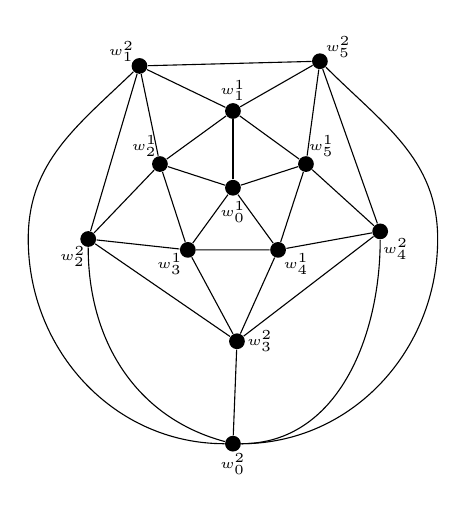
\begin{tikzpicture}[scale=1.3]
\draw (0,0) node[vx, label={[label distance=-.05cm]below:$\scriptscriptstyle{w_0^1}$}] (c) {};
%
\draw (0,0)+(18+72*1:.75 cm) node[vx, label={[label distance=-.1cm]18+72*1:$\scriptscriptstyle{w_{1}^1}$}] (c1) {};
\draw (0,0)+(18+72*2:.75 cm) node[vx, label={[label distance=-.2cm]18+72*2:$\scriptscriptstyle{w_{2}^1}$}] (c2) {};
\draw (0,0)+(18+72*3:.75 cm) node[vx, label={[label distance=-.2cm]18+72*3:$\scriptscriptstyle{w_{3}^1}$}] (c3) {};
\draw (0,0)+(18+72*4:.75 cm) node[vx, label={[label distance=-.2cm]18+72*4:$\scriptscriptstyle{w_{4}^1}$}] (c4) {};
\draw (0,0)+(18+72*5:.75 cm) node[vx, label={[label distance=-.2cm]18+72*5:$\scriptscriptstyle{w_{5}^1}$}] (c5) {};
%
\draw (0,0)+(55.5+72*1:1.5 cm) node[vx, label={[label distance=-.2cm]55.5+72*1:$\scriptscriptstyle{w_{1}^2}$}] (d1) {};
\draw (0,0)+(55.5+72*2:1.5 cm) node[vx, label={[label distance=-.2cm]55.5+72*2:$\scriptscriptstyle{w_{2}^2}$}] (d2) {};
\draw (0,0)+(55.5+72*3:1.5 cm) node[vx, label={[label distance=-.1cm]359:$\scriptscriptstyle{w_{3}^2}$}] (d3) {};
\draw (0,0)+(55.5+72*4:1.5 cm) node[vx, label={[label distance=-.2cm]55.5+72*4:$\scriptscriptstyle{w_{4}^2}$}] (d4) {};
\draw (0,0)+(55.5+72*5:1.5 cm) node[vx, label={[label distance=-.2cm]55.5+72*5:$\scriptscriptstyle{w_{5}^2}$}] (d5) {};
%
\foreach \x in {1,...,5}
    {
	\draw (c)--(c\x);
	\draw (c\x)--(d\x);}
%
\draw (c1)--(c2)--(c3)--(c4)--(c5)--(c1);
\draw (c1)--(d5);
\draw (c2)--(d1);
\draw (c3)--(d2);
\draw (c4)--(d3);
\draw (c5)--(d4);
\draw (d1)--(d2)--(d3)--(d4)--(d5)--(d1);
\draw (0,-2.5) node[vx, label={[label distance=-.1cm]below:$\scriptscriptstyle{w_0^2}$}] (d) {};
\draw (d)--(d3);
\draw (d2) to[out=-90, in=165] (d) to[out=0, in=-90] (d4);
\draw (d1) to[out=224, in=90] (-2,-.5) to[out=-90, in=180] (d) to[out=0, in=-90] (2,-.5) to[out=90,in=-45] (d5);
\end{tikzpicture}\caption{The icosahedron graph.} \label{fig:icos}
\end{centering}
\end{figure}


\begin{prop}\label{prop:C4indsat}
For $j \in \{5,6,7\}$, and $k \geq 2$, $I_j^k$ is $C_4$-induced-saturated.
\end{prop}
%\iftoggle{sub}{The proof is straightforward. We note that for $j>7$, it is possible to add an edge between two vertices on the outer cycle of one wheel without creating an induced $C_4$.}{
\begin{proof}
We first show that $I_j^k$ does not contain an induced $C_4$.  Suppose to the contrary that it does.  Since a single wheel does not contain an induced $C_4$, this $C_4$ must contain vertices from at least two different wheels.  Suppose that $w_0^p$ is in this $C_4$.  Recall that $w_0^p$ is the center of wheel $W^p$.  Then, this $C_4$ must contain $w_r^p$ and $w_s^p$ such that $|s - r| \ge 2$.  However, since $|s - r| \ge 2$, $w_r^p$ and $w_s^p$ contain no common neighbors outside of $W^p$.  Thus, all four vertices of this induced $C_4$ must be inside of $W^p$, a contradiction.  So our induced $C_4$ contains no centers of wheels.

If this $C_4$ contains exactly three vertices from a single $W^p$, then they must be consecutive along their cycle.  That is, $C_4$ contains $w_s^p, w_{s+1}^p$, and $w_{s+2}^p$.  However, as above, $w_s^p$ and $w_{s+2}^p$ have no common neighbors outside of $W^p$.  Thus, our induced $C_4$ contains at most two vertices from each $W^p$.

If this $C_4$ contains exactly two vertices from a single $W^p$, then by the same arguments used above, they must be adjacent in $W^p$, say $w_s^p$ and $w_{s+1}^p$.  No vertex of the form $w_s^q$, with $q < p$, or $w_{s+1}^r$, with $r > p$, can be in our $C_4$, as either produces a triangle with $w_s^p$ and $w_{s+1}^p$.

Now, $w_{s+1}^p$ must have another neighbor in our $C_4$.  Suppose it is in $W^t$.  If $t > p$, then it must be $w_{s+2}^t$ by the above.  However, the only common neighbors $w_{s+2}^t$ and $w_s^p$ have are of the form $w_{s+1}^q$ where $q > p$, a contradiction.  So $t < p$, and the other neighbor of $w_{s+1}^p$ is $w_{s+1}^t$.  Again though, the only common neighbors of $w_s^p$ and $w_{s+1}^t$ are either of the form $w_{s+1}^q$ where $q > p$, or $w_s^r$ where $r < p$.  In either case, we have a contradiction to the above.  Thus, our $C_4$ has exactly one vertex from each wheel.

Supose our induced $C_4$ contains the vertices $w_{t_1}^p, w_{t_2}^q, w_{t_3}^r, w_{t_4}^s$.  If $|\{t_1,t_2,t_3,t_4\}| \le 2$, then we have a triangle, a contradiction.  If $|\{t_1,t_2,t_3,t_4\}| = 4$, then some vertex is not adjacent to two of the others, a contradiction.  So $|\{t_1,t_2,t_3,t_4\}| = 3$, and two vertices have the same subscript.  We may assume that it is $w_{t_1}^p, w_{t_2}^q = w_{t_1}^q$, and that $p < q$.  Then, $w_{t_1}^p$ must have a neighbor not adjacent to $w_{t_1}^q$ in this $C_4$, say it is $w_{t_3}^r$.  However, in order for this to be possible, we must have $t_3 = t_1 + 1$ and $p < r < q$.  Thus, $w_{t_4}^s$ is adjacent to both $w_{t_1+1}^r$ and $w_{t_1}^q$.  However, since $t_4$ must be distinct from both $t_1$ and $t_1 + 1$, this cannot happen, a contradiction.  So $I_j^k$ is $C_4$-free.

By inspection we see that $I_j^k$ has the property that every edge is the lone diagonal of a $C_4$.  Thus, removing any edge results in an induced $C_4$.  So we only need to consider adding edges.  Adding an edge within one wheel (say $W^m$) is simply adding a chord $w_i^m w_p^m$ to a 5-, 6-, or 7-cycle. If $p \neq i+2$ or $j = 5$, then this chord creates an induced 4-cycle. If $p = i+2$ and $j = 6$ or $j =7$, then if $m \neq k$, $w_i^m w_{i+1}^\ell w_{i+2}^\ell w_{i+2}^m w_i^1$ is an induced 4-cycle, where $\ell > m$, and if $m = k$, then $w_i^m w_{i+1}^m w_{i+1}^\ell w_i^\ell$ is an induced $C_4$.

Now suppose we add an edge between wheels, say $W^m$ and $W^\ell$, where we may assume $m < \ell$. If the new edge is between the centers of these wheels, that is, $w_0^m w_0^\ell$, then $w_0^m w_0^\ell w_1^\ell w_1^m w_0^m$ is an induced $C_4$. If it is from the center of $W_m$ to a vertex on the cycle of $W^\ell$, say $w_i^\ell$, then $w_0^m w_i^\ell w_{i+1}^\ell w_{i+1}^m w_0^m$ is an induced $C_4$; a similar cycle is also created if the new edge is $w_0^\ell w_i^m$.
Finally, if we add an edge $w_i^m w_p^\ell$, note that $w_i^m$ is not adjacent to at least one of $w_p^m$ and $w_{p-1}^m$; label this vertex $u$. Since $u$ is adjacent to $w_{p}^\ell$, the vertices $w_0^m, w_i^m, w_p^\ell$, and $u$ induce a $C_4$.
\end{proof}
%}


%%%%%%%%%%%%%
\begin{comment}
First we will show that $I_j^k$ does not contain an induced $C_4$. A single wheel does not contain an induced $C_4$, so any $C_4$-subgraph must use vertices from at least two different wheels.
Suppose first that there is a $C_4=uxvy$ whose vertices come from only two wheels, say $W^i$ and $W^p$.
First suppose that $u$ is the center of $W^i$. % a wheel, say $W^1$.
Then $v$ must be in $V(W^p)$ and $x$ and $y$ must be in $V(W^i)$.
The neighbors of $v$ on $W^i$ are all adjacent, so $x$ and $y$ must be adjacent, and thus the four vertices do not induce a $C_4$. If $u$ and $v$ are both not centers of a wheel, then suppose they are both in (but not the center of) the same wheel, say $W^i$. In this case, one of $x$ or $y$ must be $w_0^i$, and the other must also be on $W^i$, which means that $x$ and $y$ are adjacent and these vertices do not create an induced $C_4$. Finally, consider the case where $u$ and $v$ are on (but not the centers of) different wheels. In this case, $x$ and $y$ must be on different wheels as well; suppose $u$ and $x$ are on $W^i$ and $v$ and $y$ are on $W^p$. Then, since $u$ is adjacent to $y$ and the neighbors of $y$ on $W^i$ must be adjacent, we have $x$ adjacent to $y$, so that $\{u,v,x,y\}$ does not induce a $C_4$.

Now consider the case where the four vertices of a $C_4$ are on three different wheels in $I_j^k$ (assuming $k \ge 3$). In this case, none of these vertices can be the centers of a wheel, because that would require three vertices from the same wheel.
Without loss of generality, suppose $W^i$ contains two vertices of this $C_4$, and they are $w_3^i$ and $w_4^i$. Let $W^\ell$ and $W^p$ be the remaining wheels. Then the neighbor of $w_3^i$ on $W^\ell$ is either $w_2^\ell, w_3^\ell$, or $w_4^\ell$ and the neighbor of $w_4^i$ on $W^p$ is either $w_3^p, w_4^p$, or $w_5^p$. However, we can eliminate $w_4^\ell$ and $w_3^p$ from these options, because otherwise our $C_4$ would have a chord. Since the vertices of the $C_4$ on $W^\ell$ and $W^p$ must be adjacent, we then see that they must be $w_3^\ell$ and $w_4^p$. This means that $\ell < p$. If $i < p$, then the $C_4$ has the chord $w_3^i w_4^p$, and if $i > \ell$, the $C_4$ has the chord $w_3^\ell w_4^i$.
Either way the $C_4$ is not induced.

Finally, if the four vertices of a $C_4$ come from four different wheels, say $W^i, W^\ell, W^m$, and $W^p$, where $i < \ell < m < p$. Again, none of the vertices of a $C_4$ can be the centers of the wheels.
If the vertex from $W^i$ is $w_r^i$, then the remaining vertices all have index (subscript) $r$ or $r+1$.
If three of the vertices have the same index, then those three vertices form a triangle and the $C_4$ is not induced.
So two of them have index $r$ (and thus cannot be from $W^p$) and the other two have index $r+1$.
This means the cycle must be on the vertices $w_r^i, w_{r+1}^p, w_{r+1}^m$, and $w_r^\ell$, but these vertices do not create an induced $C_4$. Thus, $I_j^k$ does not contain an induced $C_4$.

Note that $I_j^k$ is a triangulation, so removing any edge changes two 3-faces into one 4-face, or an induced $C_4$.
We then only need to show that adding an edge creates an induced 4-cycle.
Adding an edge within one wheel (say $W^m$) is simply adding a chord $w_i^m w_p^m$ to a 5-, 6-, or 7-cycle. If $p \neq i+2$ or $j = 5$, then this chord creates an induced 4-cycle. If $p = i+2$ and $j = 6$ or $j =7$, then if $m \neq k$, $w_i^m w_{i+1}^\ell w_{i+2}^\ell w_{i+2}^m w_i^1$ is an induced 4-cycle, where $\ell > m$, and if $m = k$, then $w_i^m w_{i+1}^m w_{i+1}^\ell w_i^\ell$ is an induced $C_4$.

Now suppose we add an edge between wheels, say $W^m$ and $W^\ell$, where we may assume $m < \ell$. If the new edge is between the centers of these wheels, that is, $w_0^m w_0^\ell$, then $w_0^m w_0^\ell w_1^\ell w_1^m w_0^m$ is an induced $C_4$. If it is from the center of $W_m$ to a vertex on the cycle of $W^\ell$, say $w_i^\ell$, then $w_0^m w_i^\ell w_{i+1}^\ell w_{i+1}^m w_0^m$ is an induced $C_4$; a similar cycle is also created if the new edge is $w_0^\ell w_i^m$.
Finally, if we add an edge $w_i^m w_p^\ell$, note that $w_i^m$ is not adjacent to at least one of $w_p^m$ and $w_{p-1}^m$; label this vertex $u$. Since $u$ is adjacent to $w_{p}^\ell$, the vertices $w_0^m, w_i^m, w_p^\ell$, and $u$ induce a $C_4$.


\end{comment}
%%%%%%%%%%%%%%



Proposition \ref{prop:C4indsat} implies that for many values of $n$, $\indsat{n}{C_4}=0$. In fact, this is the case for $n \geq 12$. To show this, we use the following proposition regarding $kK_2$.  While we only employ the proposition in the case $k = 2$, the more general statement which we present is not difficult.


\begin{prop}\label{twins matching}
Let $s:=(s_1,\dots, s_n)$ be a sequence of positive integers.  Let $G$ be a graph with vertex set $\{v_1,\ldots v_n\}$, and let $G_s$ be the graph obtained from $G$ by replacing each vertex $v_i$ with an independent set of order $s_i$ and each edge with a complete bipartite graph between the corresponding independent sets.
For $k \ge 2$, $G$ is $kK_2$-induced-saturated if and only if $G_s$ is  $kK_2$-induced-saturated.
\end{prop}


%\iftoggle{sub}{The proof is straightforward.}{
\begin{proof}
For each vertex $v_i \in V(G)$, let $V_i$ be the independent set in $G_s$ that corresponds to it.
We will call this collection of vertices in $G_s$ that replaces a single vertex in $G$ a \emph{part}.

Note that %since no two vertices in a matching share the same neighborhood,
no induced matching in $G_s$ uses two vertices from the same part, and the same holds if we add or remove a single edge from $G_s$.
We claim that if $w_i$ and $w_j$ are vertices from different parts $V_i$ and $V_j$, respectively, of $G_s$, then $G_s$ (or  $G_s+w_iw_j$ or $G_s-w_iw_j$) contains an induced matching %that uses no two vertices in the same part
if and only if $G$ (resp. $G+v_iv_j$, or $G-v_iv_j$) contains an induced matching $M$.
Suppose $M_s$ is such an induced matching in $G_s$ (or $G_s+w_iw_j$ or $G_s-w_iw_j$). Then each vertex in $M_s$ comes from a different part of $G_s$ (resp. $G_s+w_iw_j$ or $G_s-w_iw_j$), and thus they correspond to distinct vertices in $V(G)$.
%each of which is only adjacent to the vertex corresponding to the one it was adjacent to in $M_s$.
This is an induced matching in $G$.

If $G$ (or $G+v_iv_j$ or $G-v_iv_j$) has an induced matching $M$, then when the graph is expanded, no new adjacencies have been added between the parts corresponding to the endpoints of vertices in $M$ (except for $w_iw_j$ in the case of $G+v_iv_j$).  Thus, we can find an induced matching in $G_s$ (resp. $G_s+w_iw_j$ or $G_s-w_iw_j$).
This shows that if $G_s$ is $kK_2$-induced-saturated, then so is $G$.

To show that if $G$ is $kK_2$-induced-saturated, then so is $G_s$, it remains to consider adding edges between vertices in one part of $G_s$.  First we note that $G$ has no dominating vertex. Indeed, if $u$ is a dominating vertex, then deleting an edge incident to $u$, say $uw$, does not create an induced $2K_2$, let alone an induced $kK_2$, as $u$ dominates $N_G(w)$.

Now, suppose we add $w_iw_i'$ to $G_s$, in the part $V_i$ corresponding to $v_i$.
Since $v_i$ is not dominating, there exists $w$ not adjacent to $v_i$.  Since $G$ is $kK_2$-induced-saturated, $G+v_iw$ contains an induced matching $M=\{v_iw,x_2y_2,\ldots,x_ky_k\}$. Then $M_s=\{w_iw_i',X_2Y_2,\ldots,X_kY_k\}$ is an induced matching in $G_s+w_iw_i'$, where $X_j$ and $Y_j$ are vertices in the parts corresponding to $x_j$ and $y_j$, respectively.
\end{proof}
%}


\begin{cor}
For $n \ge 12$, $\indsat{n}{C_4} = 0$.
\end{cor}

\begin{proof}
Applying Observation \ref{thm:complement} to case $k = 2$ in Proposition \ref{twins matching}, allows us to begin with a graph that is $C_4$-induced-saturated, replace a single vertex with a clique of any order, replace the affected edges with complete bipartite graphs, and produce another graph that is $C_4$-induced-saturated.  Thus, beginning with $I_5^2$, applying these operations obtains $C_4$-induced-saturated graphs for all values of $n \ge 12$.
\end{proof}

%%%%%%%%%%
\begin{comment}
Recall that Observation \ref{thm:complement} states that a graph is $H$-induced-saturated if and only if its complement is $\overline{H}$-induced-saturated.
Thus, beginning with a graph that is $C_4$-induced-saturated, the operations of replacing a single vertex with a clique of some order and replacing the affected edges with complete bipartite graphs produces another graph that is $C_4$-induced-saturated.
This shows that we can create $C_4$-induced-saturated graphs for any $n \geq 12$ by applying these operations to the graphs in Construction \ref{gen gen icos}. Thus, $\indsat{n}{C_4} =0$ for all $n \ge 12$.
\end{comment}
%%%%%%%%%%%

For $4 \le n \le 10$, a computer search showed $\indsat{n}{C_4} > 0$.  At this time, whether $\indsat{11}{C_4}$ is zero or not, is yet unknown.  We now turn our attention to $\sis{n}{C_4}$.
%Now that we have shown that $\indsat{n}{C_4}=0$ for $n \ge 12$, we turn our attention to computing $\sis{n}{C_4}$.

\begin{thm}\label{prop:C4}
For sufficiently large $n$, $(5/2)n \leq \sis{n}{C_4}\leq (7/64)n^2+o(n)$.
\end{thm}
\begin{proof}
To prove the lower bound we show that $\delta(G) \ge 5$.
Suppose $G$ is a $C_4$-induced-saturated graph.
Let $x \in V(G)$, and let $H:=G[N(x)]$.  Since deleting any edge produces an induced $C_4$, every edge is the diagonal of a $C_4$ and $\deg(x) \ge 3$.  In particular, there exists $v_1,v_2,v_3 \in V(H)$ such that $v_1v_3$ is not an edge, but $v_1v_2$ and $v_2v_3$ are edges.  Now, $G - xv_1$ contains an induced $C_4$ that contains both $x$ and $v_1$, but not $v_3$.  If $v_2$ is not in this $C_4$, then there exists two other vertices distinct from $v_1,v_2,v_3$ in $H$.  Thus, $\deg(x) \ge 5$.  If $v_2$ is in this $C_4$, then there exists $v_4 \in V(H)$  distinct from $v_1,v_2,v_3$ such that $v_1v_4$ is an edge, but $v_2v_4$ is not.  By a similar argument, considering $G - xv_3$ gives at least one additional vertex in $H$ distinct from $v_1,v_2,v_3,v_4$.  So in any case, $\deg(x) \ge 5$, and as $x$ was arbitrary, $\delta(G) \ge 5$.  Thus, provided $n \ge 12$, $\sis{n}{C_4} \ge (5/2)n$.


%Starting with the icosahedron, applying Proposition~\ref{twins matching} and complementation yields a $C_4$-induced-saturated graph of order $n$, for any $n \ge 12$, that has minimum degree at least 5. Thus, $(5/2)n \leq \sis{n}{C_4}$ for every $n \ge 12$.
%%%this was already mentioned in the discussion following 5.3 AND 5.2

To prove the upper bound, we choose $n \geq 56$ and create a graph $G$ of order $n$. Let $r \equiv n \mod 8$, where $0 \le r \le 7$.  Set $k=\lfloor n/8 \rfloor$ so that $k \ge r$ and $n(I_7^k)=8k$.  If $r=0$, choose $G=I_7^k$. If $r>0$, we create $G$ by adding $r$ vertices to $I_7^k$. Recall, as discussed after Proposition~\ref{twins matching},
by replacing the vertices of $I_7^k$ with cliques, and its edges with complete bipartite graphs,
we preserve the property of being $C_4$-induced-saturated.
Accordingly, using the notation of Construction~\ref{gen gen icos}, we replace $w_0^1,\ldots, w_0^r$ with copies of $K_2$ and make each new vertex adjacent to the neighborhood of the vertex it replaces.

Now we determine $e(G)$. The first $r$ wheels have $22$ edges, and the rest have $14$. Between any two wheels there are $14$ edges. So $e(G)=14\left[{k \choose 2}+k\right]+8r$. Since
$r \in [0,7]$ and $k=\lfloor n/8 \rfloor$, $e(G) \leq \frac{7}{64}n^2+\frac{7}{8}n+56$.

%Then each edge of $I_j^k$ is replaced by $\left(\displaystyle\frac{n}{(j+1)k}\right)^2$ edges, and each vertex of $I_j^k$ is a clique of order $\frac{n}{(j+1)k}$ in $G$.  gives rise to approximately $\displaystyle\frac{1}{2}\left(\displaystyle\frac{n}{(j+1)k}\right)^2$ edges, so
%\begin{align*}
%e(G) \approx~&\|I_j^k\|\left(\frac{n}{(j+1)k}\right)^2+|I_7|\frac{1}{2}\left(\frac{n}{(j+1)k}\right)^2\\
% =~&jk(k+1)\left(\frac{n}{(j+1)k}\right)^2+(j+1)k\frac{1}{2}\left(\frac{n}{(j+1)k}\right)^2\\
% =~&n^2\left( \frac{j}{(j+1)^2}+\frac{3j+1}{2k(j+1)^2}\right).
% \intertext{For fixed $j$, this quantity is minimized by taking $k$ as big as possible; that is, $k=n/(j+1)$, and (modulo a few stray vertices to make parity work out) $G=I_j^{n/(j+1)}$. Then,}
% e(G)=~&\|I_j^{n/(j+1)}\| = j\left(\frac{n}{j+1}\right)\left(\frac{n}{j+1}+1\right)\\
% \approx~&j\left(\frac{n}{j+1}\right)^2.
% \intertext{For $j=7$, this yields}
%  e(G)=~&\frac{7}{64}n^2 \approx 0.109n^2.
% \end{align*}
\end{proof}

\subsection{Matchings}
Another graph that is $C_4$-induced-saturated is the join $I_5^2 \vee K_{n-12}$.
Observation \ref{thm:complement} implies that the complement of this graph is $2K_2$-induced-saturated. We can further generalize this to get a $kK_2$-induced-saturated graph for any $k\geq 2$.

\begin{prop}\label{clm:match}
Let $\overline{I_5^2}$ be the complement of the icosahedron. For fixed $k$ and $n \geq 12(k-1)$, the graph $(k-1)\overline{I_5^2} + (n-12(k-1))K_1$ is $kK_2$-induced-saturated. Thus, for $n \geq 12(k-1)$, $\indsat{n}{kK_2}=0$.
\end{prop}
%\iftoggle{sub}{The proof is straightforward.}{
\begin{proof}
By Proposition~\ref{prop:C4indsat} and Observation~\ref{thm:complement}, the complement of an icosahedron is $2K_2$-induced-saturated. Let $G$ denote $(k-1)\bar{I_5^2} + (n - 12(k - 1))K_1$.  Clearly, $G$ contains $(k-1)K_2$ as an induced subgraph, but no induced $kK_2$.  If we add or delete any edge inside a component, or add an edge among the isolates, we create an induced $kK_2$. Note that every vertex $v$ in $\bar{I_5^2}$ is in an induced copy of $K_2+K_1$ where $v$ is the isolate.  Thus, adding any edge with an endpoint in a copy of $\bar{I_5^2}$ creates an induced $kK_2$.
\end{proof}
%}


%An immediate corollary of Proposition \ref{clm:match} is an upper bound on $\sis{n}{kK_2}$ for any $n \ge 12(k-1)$.

\begin{cor} For $n\geq 12(k-1)$, $\sis{n}{kK_2} \leq 36(k-1)$.
\end{cor}
In particular, for fixed $k$, $\sis{n}{kK_2}$ is constant.


%%%%%%%%%%%%%%%%%%%%%%%%%%%%%%%
%
%                  ODD CYCLES ET AL
%
%%%%%%%%%%%%%%%%%%%%%%%%%%%%%%%


\section{Other Cycles and Generalizations of Cycles}

In this section we provide a construction proving that odd cycles also have induced saturation number zero for $n$ sufficiently large.  As it is already known that  $\indsat{n}{C_3} = \sat{n}{C_3}$ \cite{MS}, we only consider odd cycles of length at least five.  Additionally,  this construction is also $H$-induced-saturated when $H$ is a modification of an even cycle as described below.

Let $C_{2k}'$ denote a cycle of length $2k$ with a pendant vertex, and $\hat C_{2k}$ denote an even cycle with a chord between two vertices at distance 2 from each other (sometimes called a triangle chord or hop).

For a given $k$ and $n \geq (k+1)^2+2$, we can write $n$ as $(k+1)t-s$ where $t$ and $s$ are integers with $t \geq k+2$ and $0 \leq s \leq t-3$.
In particular, we choose $t=\cl{\frac{n}{k+1}}$.
Using this expression for $n$, we give the following construction.

\begin{cons}\label{cons:cycles}
For $k \geq 3$ and $n \geq (k+1)^2+2$, let $n=(k+1)t-s$, where $t=\cl{\frac{n}{k+1}} \ge k+2$ and $0 \leq s \le t-3$.
Let $G_{n,k}$ be formed from the Cartesian product $K_{k+1} \cartprod K_t$ by removing $s$ vertices from one copy of $K_t$.
\end{cons}

\begin{prop}\label{indsat_cycles}
If $H \in \{C_{2k-1}, C_{2k}', \hat C_{2k}\}$, then the graph $G_{n,k}$ in Construction \ref{cons:cycles} is $H$-induced-saturated.
\end{prop}
%\iftoggle{sub}{We omit the proof.}{
\begin{proof}
Let $G_{n,k}$ be as described in Construction \ref{cons:cycles}.  We first show that $G_{n,k}$ is $H$-free for $H \in \{C_{2k-1}, C_{2k}', \hat C_{2k}\}$.  Any induced subgraph of $G_{n,k}$ that is triangle-free has at most two vertices from any copy of $K_{k+1}$ or $K_t$.
Since $2k-1$ is odd, an induced $C_{2k-1}$ would contain precisely one vertex $v$ from some copy of $K_{k+1}$. Then the neighbors of $v$ must be in the same copy of $K_t$, which means they form a triangle. Thus, $G_{n,k}$ has no induced odd cycle larger than a triangle.  Since $\hat C_{2k}$ contains $C_{2k-1}$ as an induced subgraph, neither $C_{2k-1}$ nor $\hat C_{2k}$ are induced subgraphs of $G_{n,k}$.  Similarly, if $G_{n,k}$ contained an induced $C'_{2k}$, then because $C'_{2k}$ is triangle-free with an odd number of vertices, then there would be one copy of $K_t$ that contains precisely one vertex $v$ of the subgraph. If $v$ is on the cycle, it has at least two neighbors, but these can only be other copies of $v$, forming a triangle in some copy of $K_{k+1}$. If $v$ is the pendant vertex, suppose it has neighbor $u$ on the cycle. Then $u$ has some neighbor $u'$ in a different copy of $K_t$ from itself, and $u,u'$, and $v$ are all in one copy of $K_{k+1}$, forming a triangle. Thus, $G_{n,k}$ has no induced $C'_{2k}$.

In the remainder of this proof we view $K_{k+1} \cartprod K_t$ as a $k+1$ by $t$ grid with vertices $v_{i,j}$ for $1 \le i \le k+1$ and $1 \le j \le t$, and the graph induced by the vertices a row (or column) is a clique.  In particular, we have $k+1$ columns and $t$ rows.  We then form $G_{n,k}$ by removing $s$ vertices from a copy of $K_t$, and let $K_t^*$ denote the clique induced by the remaining $t - s$ vertices.
%Then, form $G_{n,k}$ by removing $v_{i, k+1}$ for $t-s+1 \le i \le t$.
Since $s \le t-3$ and $k \ge 3$, $G_{n,k}$ has at least three vertices in each row and column, and at least three rows with at least 4 vertices.

Let $G_{n,k}'$ be obtained from $G_{n,k}$ by adding an edge.  Up to relabeling, we may assume that $v_{1,1}v_{k+1,k+1}$ is the added edge, and $v_{1,1}$ is not in $K_t^*$.  Suppose first that $v_{k+1,k+1}$ is in $K_t^*$ (i.e., the $(k+1)$st column induces $K_t^*$).  Let $T := \{v_{i,i+1}, v_{i+1,i+1}: 1 \le i \le k-2\} \cup \{v_{1,1}, v_{k+1,k+1}\}$.  Then $T \cup \{v_{k-1,k+1}\}$ induces $C_{2k-1}$, $T \cup  \{v_{k-1,k},v_{k-1,k+1}\}$ induces $\hat C_{2k}$, and $T \cup \{v_{k-1,k}, v_{k,k}, v_{k,1}\}$ induces $C_{2k}'$.

If $v_{k+1,k+1}$ is not in $K_t^*$, then we can switch the column containing $K_t^*$ with the $k$th column and relabel the vertices appropriately.  Note that $v_{1,1}v_{k+1,k+1}$ is still the added edge as $K_t^*$ is not in the first or $(k+1)$st column.
  In this case, we find an induced $C_{2k-1}$ and $\hat C_{2k}$ from the same sets used above.  In order to find an induced $C_{2k}'$, we consider the vertices in $K_t^*$.  Since $t - s \ge 3$, $K_t^*$ contains a vertex not in the first or $(k+1)$st column.  Up to permuting rows 2 through $k$ and relabeling vertices, we may assume that $v_{k,k}$ is such a vertex.  If $v_{k,k+1}$ is also a vertex in $K_t^*$, then $(T\setminus\{v_{1,2}\}) \cup \{v_{k+1,2}, v_{k,k+1}, v_{k,k}, v_{k-1,k}\}$ induces $C_{2k}'$.  If not, then $K_t^*$ contains two vertices not in the first or $(k+1)$st row, and up to permuting rows 2 through $k-1$ and relabeling vertices, we may assume that $v_{k,k-1}$ is such a vertex.  Then $\{v_{i,i}, v_{i+1,i}: 2\le i \le k\} \cup \{v_{2,k+1}, v_{k+1,k+1}, v_{1,1}\}$ induces $C_{2k}'$.

Now let $G_{n,k}'$ be obtained from $G_{n,k}$ by deleting an edge.  Again, up to relabeling, we may assume that either $v_{1,1}v_{1,2}$  or $v_{1,1}v_{2,1}$ is the deleted edge.

Suppose first that $v_{1,1}v_{1,2}$ is the deleted edge.  If this edge was in $K_t^*$, we can switch rows and relabel the vertices so that $v_{1,1}, v_{1,2}$, and $v_{1,k+1}$ are in $K_t^*$.  If not $v_{1,1}v_{1,1}$ is not in $K_t^*$, then switch the column containing $K_t^*$ with the $(k+1)$st column and relabel the vertices.  Note that $v_{1,1}v_{1,2}$ is still the deleted edge.  For $T$ as defined above, $T \cup \{v_{k-1,1}\}$ induces $C_{2k-1}$, $T \cup \{v_{k-1,1}, v_{k-1,k}\}$ induces $\hat C{2k}$, and $T \cup \{v_{k-1,k}, v_{k,k}, v_{k,k+1}\}$  induces $C_{2k}'$.

Now suppose that $v_{1,1}v_{2,1}$ is the deleted edge, and without loss of generality,  $v_{1,1}$ is not in $K_t^*$.  If $v_{2,1}$ is in $K_t^*$, then we can switch rows and relabel vertices so that $v_{2,2}$ exists.  If $v_{2,1}$ is not in $K_t^*$, then we switch the column containing $K_t^*$ with the $(k+1)$st column.  Note that $K_t^*$ contains at least two vertices not in the first row so that up to permuting rows 2 through $k+1$ and relabeling vertices, we may assume $v_{k+1,k-1}$ and $v_{k+1,k}$ exist.  In either case, the deleted edge is still $v_{1,1}v_{2,1}$.  Let $T' := \{v_{i+1,i}, v_{i+1,i+1}: 1 \le i \le k - 2\} \cup \{v_{1,1}\}$.  Then $T \cup \{v_{1,k-1}, v_{k,1}\}$ induces $C_{2k-1}$, $T \cup \{v_{1,k-1}, v_{1,k}, v_{k,1}\}$ induces $\hat C_{2k}$, and $T \cup \{v_{k+1,k-1}, v_{k+1,k}, v_{k,k}, v_{k,1}\}$ induces $C_{2k}'$.
%
%Now suppose the edge $v_{i,j}v_{i,j+1}$ is deleted from $G_{n,k}$; call this graph $G_{n,k}'$.
%We will consider all addition and subtraction to be done modulo the length of the row or column (that is, if row $i$ has $k+1$ vertices, then $v_{i,k+2}=v_{i,1}$, and if row $i$ has $k$ vertices, then $v_{i,k+1}=v_{i,k}$).
%Note that the vertices $\{v_{i,j}, v_{i, j+2},v_{i,j+1}\}$ induce a $P_3$ in $G_{n,k}'$, and this will enable us to find induced copies of $C_{2k-1}$, $C_{2k}'$, and $\hat C_{2k}$.
%Consider the vertex set $$T=\{v_{i,j}, v_{i, j+1}, v_{i, j+2}, v_{i+1, j}, v_{i+1, j+3}, v_{i+2, j+3}, v_{i+2, j+4}, \ldots v_{i+k-2,j+k-1}, v_{i+k-2, j+1}\}.$$
%
%This set contains $2k-1$ vertices, with two vertices each from columns $i+1$ through $i+k-2$ and rows $j$, $j+1$, and $j+3$ through $j+k-1$; three vertices from column $i$; and one vertex from row $j+2$. At most $k$ columns and $k$ rows are represented, and since there are at least $k$ rows and columns, this set of vertices can be found. If column $i+1$ does not have 4 vertices in it, then replace that column with one that does, so that $v_{i+1,j+3}\neq v_{i+1,j}$.
%The set $T$ induces the odd cycle $C_{2k-1}$.
%If we add the vertex $v_{i+k-2,j+k-1}$ to $T$, creating a set $T'$, then $T'$ induces $\hat C_{2k}$.
%Finally, if we let $T''=(T\setminus\{v_{i+1,j}\})\cup \{v_{i+1,j+2}\}$, then $T''$ induces $C_{2k}'$.
%
%If we remove the edge $v_{i, j} v_{i+1, j}$ instead, then a similar construction works. Up to renaming the vertices, all edges in $G_{n,k}$ are of these two forms.
%
%Adding an edge works similarly.
\end{proof}
%}

\begin{cor}\label{cor:cycles}
For all $k \geq 3$, if $n \geq (k+1)^2+2$ and $H\in\{C_{2k-1},C_{2k}',\hat C_{2k}\}$, then $\indsat nH =0$.
\end{cor}

In the following discussion assume $H \in \{C_{2k-1}, C_{2k}', \hat C_{2k}\}$.  Using Construction \ref{cons:cycles} we obtain an upper bound on $\sis{n}{H}$ with order of magnitude $n^2$, which is trivial.  We can improve this order of magnitude slightly in the case when $\lceil \sqrt{n}~ \rceil$ is not prime.  To do so we note that if $n$ can be written as a product of two integers $s$ and $t$ that are both at least $k$, then the graph $K_s \cartprod K_t$ is $H$-induced-saturated.


\begin{prop}
Fix $k \ge 3$ and choose $n$ such that $n^{1/4} \ge k + 1$.  For $H \in \{C_{2k-1}, C_{2k}', \hat C_{2k}\}$, if $\lceil \sqrt{n}~ \rceil$ is divisible by some $t \ge 3$, $\sis{n}{H} \le cn^{7/4} + O(n^{3/2})$ for some constant $c$.
\end{prop}

\begin{proof}
As noted above, the Cartesian product of two sufficiently large cliques is $H$-induced-saturated.  So, consider $G := K_{\lceil \sqrt{n}~\rceil/t} \cartprod K_{t\lceil \sqrt{n}~ \rceil}$.  Simple computation shows $n \le v(G) \le n + 2\sqrt{n} + 1$.  So, $n(G)$ can be written as $n + s$, where $0 \le s \le 2\sqrt{n} + 1 \le t\sqrt{n} - 3$, as $t \ge 3$.  Let $G'$ be obtained from $G$ by removing $s$ vertices from a single copy of $K_{3\lceil \sqrt{n}~\rceil}$ as in Construction \ref{cons:cycles}.  An argument similar to that in Proposition \ref{indsat_cycles} shows that $G'$ is $H$-induced-saturated.  Observe: $$e(G') \le t\lceil\sqrt{n}~\rceil \binom{(1/t)\lceil \sqrt{n}~\rceil}{2} + (1/t)\lceil\sqrt{n}~\rceil \binom{t\lceil \sqrt{n}~\rceil}{2} = \frac{\lceil \sqrt{n}~\rceil^2}{2}\left(\left(t+\frac{1}{t}\right)\lceil\sqrt{n}~\rceil) - 2\right).$$
Since $t$ divides $\lceil\sqrt{n}~\rceil$, $t \le \sqrt{\lceil \sqrt{n}~\rceil}\le c'n^{1/4}$ for some $c' > 1$.  Using this and $\lceil\sqrt{n}~\rceil \le \sqrt{n} + 1$ gives $e(G') \le \frac{c'}{2}n^{7/4} + O(n^{3/2})$.
\end{proof}


Considering odd cycles  points out another property of the induced saturation number.
That is, if $\indsat{n}{H}=0$ for a particular $n$, it is not necessarily the case that $\indsat{k}{H}=0$ for all $k > n$. For example,  Construction~\ref{cons:cycles} shows $\indsat{n}{C_5}=0$ for $n = 9$ and $n \geq 12$.
However, a computer search showed that for $n=10$ and $n=11$, we have $\indsat{n}{C_5} > 0$.
(A $C_5$-induced-saturated trigraph on 10 vertices with one gray edge is shown in Figure \ref{fig:C5_10}, so that $\indsat{10}{C_5}=1$.)
%Thus, we have an example of a graph $H$ for which $\indsat{n}{H} =0$ but $\indsat{n+1}{H}\neq 0$.


%\begin{prop}
%For fixed $k \ge 3$ and $n \ge (k+1)^2+2$, $\frac{3}{2}n \le \sis{n}{H} \le n^{3/2}$, where $H \in \{C_{2k-1}, C_{2k}', %\hat{C_{2k}}\}$.
%\end{prop}

%%%%%%%%%%%%%%%%%%%%%%%%%

\begin{figure}[h]
\centering
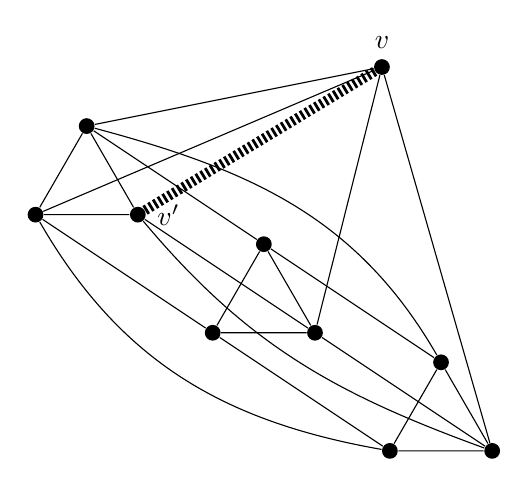
\begin{tikzpicture}[scale=0.75]
\foreach \y in {1,2,3}
	{\foreach \x in {1,2,3}
	{\draw (-3*\y,2*\y)+(90+120*\x:1cm)
	node[vx] (t\y\x){};}
	\draw (t\y1)--(t\y2)--(t\y3)--(t\y1);}
\draw (t11)--(t21)--(t31);
\draw (t31) to[out=-60, in=170] (t11);
\draw (t13)--(t23)--(t33);
\draw (t33) to[out=-15, in=120] (t13);
\draw (t32)--(t22)--(t12);
\draw (t32) to[out=-50, in=160] (t12);
\draw (-4,8) node[vx, label=above:$v$] (v){};
\draw (t31)--(v)--(t33);
\draw (t22)--(v)--(t12);
\draw (t32) node[label= right:$v'$]{};
\draw [line width=3.6pt,dash pattern=on 1pt off 1pt]  (t32) -- (v);
\end{tikzpicture}%\includegraphics[scale=.4]{figures/c5_10}
\caption{This trigraph, with the gray edge $vv'$, is a $C_5$-induced-saturated trigraph.}
\label{fig:C5_10}
\end{figure}


%%%%%%%%%%%%%%%%%%%%%%%%%%%%%
%
%               FAMILIES OF GRAPHS
%
%%%%%%%%%%%%%%%%%%%%%%%%%%%%%


\section{Families of Graphs}\label{sec:families}

In this section we extend the definition of induced saturation in \cite{MS} to families of graphs in the natural way.

\begin{defn}
For a family $\mathcal F$ of graphs, a trigraph $T$ is \textbf{$\mathcal F$-induced-saturated} if no realization of $T$ contains any member of $\mathcal F$ as an induced subgraph, but whenever any black or white edge of $T$ is turned to gray, some member of $\mathcal F$ occurs as an induced subgraph of some realization.

The \textbf{induced saturation number} of $\mathcal F$ with respect to $n$, written $\indsat{n}{\mathcal F}$, is the minimum number of gray edges in an $\mathcal{F}$-induced-saturated trigraph with $n$ vertices.
\end{defn}


For any family $\mathcal F$ containing all graphs on $k$ vertices,
 $\indsat{n}{\mathcal F}={n \choose 2}$.

Construction~\ref{cons:cycles} and Proposition~\ref{indsat_cycles} demonstrate that for any family $\mathcal F$, all of whose elements are odd cycles, even cycles with a pendant, or even cycles with a triangle chord, $\indsat{n}{\mathcal F}=0$ for $n$ sufficiently large.
However, we could have $\indsat{n}{\mathcal{F}}\neq 0$ even if there is some $G\in \mathcal{F}$ such that $\indsat{n}{G}=0$
%; for instance, any family containing $K_2$ trivially has induced saturation number zero.
%Moreover, it is possible for a graph to have induced saturation number zero, but appear in a family with nonzero induced saturation number,
as demonstrated in Proposition~\ref{threshold} below.
One may suspect this is because of the presence of $P_4$, which has nonzero induced-saturation number, yet
it is also possible for a family $\mathcal F$ to consist of graphs that each individually have induced saturation number zero, while the induced saturation number of $\mathcal F$ is nonzero. We provide an example of this in Proposition~\ref{split}.

\begin{prop}\label{threshold}
For all $n$, $\indsat{n}{\{2K_2,P_4,C_4\}} \neq 0$.
\end{prop}
\begin{proof}
The graphs that contain no induced $2K_2,P_4,$ or $C_4$ are precisely the \emph{threshold graphs} \cite{CH}. These graphs are characterized in a second way: they are constructed by iteratively adding a vertex to a graph either as an isolate or a dominating vertex. Thus, an $n$-vertex threshold graph can be represented as a string of $n$ symbols from $\{-,+\}$ as follows:
on the vertex set $V=\{v_1,\ldots,v_n\}$, for every $i>j$, $v_iv_j$ is an edge if and only if the $i$th symbol in the string is $+$.

We claim that for any threshold graph $G$ with at least one edge, there exists $e \in E(G)$ such that $G-e$ is also threshold. Let $\pi=s_1, \ldots, s_n$ be a string of symbols from $\{-,+\}$ representing $G$. Suppose there exists $i \in [n-1]$ such that $s_i=-$ and $s_{i+1}=+$, and let $i$ be minimal with this property. Then the graph $G'=G-v_iv_{i+1}$ is represented by the symbol list
$\pi'=s_1 \ldots s_{i-1}s_{i+1}s_is_{i+1}\ldots s_n$, so $G'$ is threshold.
If no such index $i$ exists, then $\pi$ is a list consisting only of $+$, so $G$ is the complete graph $K_n$; however, $K_n-e$ is also threshold.

Thus, for any graph $G$ with no induced $2K_2$, $P_4$, or $C_4$, there exists an edge $e \in G$ such that $G-e$ also has no induced $2K_2$, $P_4$, or $C_4$.
It follows that $\indsat{n}{\{2K_2,P_4,C_4\}} \neq 0$.
\end{proof}

The family of {\it split graphs} is another family of graphs that can be characterized by a set of forbidden induced subgraphs. A split graph is a graph whose vertex set can be partitioned into a clique and an independent set. F\"oldes and Hammer~\cite{FH} showed that a graph is a split graph if and only if it contains no induced $2K_2$, $C_4$, or $C_5$.

\begin{prop}\label{split}
For all $n$, $\indsat{n}{\{2K_2,C_4,C_5\}} \neq 0$.
\end{prop}
\begin{proof}
Since adding or deleting an edge between the clique part and the independent set of a split graph still results in a split graph, it follows that $\indsat{n}{\{2K_2, C_4, C_5\}} \neq 0$.
\end{proof}

We have shown that $\indsat{n}{2K_2}$, $\indsat{n}{C_4}$, and $\indsat{n}{C_5}$ are all equal to zero for sufficiently large $n$. Thus, this example shows that even though every graph in a family has induced-saturation number zero, the family itself may not have induced-saturation number zero.

%\begin{ques}
%There exist many important graph families characterized by a set $\mathcal F$ of forbidden induced subgraphs. Determine .
%\end{ques}
%In Section~\ref{sec:families}, we discussed the values of $\mathcal F$ characterizing threshold graphs and split graphs.
Other families characterized by a (not necessarily finite) family of forbidden induced subgraphs include
%comparability graphs \cite{}, %too hard!!!
perfect graphs \cite{CRST},
trivially perfect graphs \cite{W}, \cite{G},
interval graphs \cite{LB}, %"asteroidal triples" are an infinite family; also chordal implies forbidden infinite family
and line graphs \cite{B}.
It would be interesting to determine $\indsat{n}{\mathcal F}$ and $\sis{n}{\mathcal F}$ for these families. We suspect that doing so will be much more difficult than for threshold and split graphs, as the families of forbidden graphs are significantly more complicated.

%%%%%%%%%%%%%%%%%%%%%%%%%%%%%%%%%%%%%%%%%%%%%%%%%%%%%%%%%%%%%



%%%%%%%%%%%%%%%%%%%%%%%%%%%%%%%%%%%%%%%%%%%%%%%%%%%%%%%%%%%%%
%%%%%%%%%%%%%%%%%%%%%%%%%%%%%%%%%%%%%%%%%%%%%%%%%%%%%%%%%%%%%

\begin{comment}
\section{Questions and Directions}\label{sec:questions}
We list here several open questions about induced saturation and some comments.
\begin{ques}
Characterize graphs $H$ such that $\indsat{n}{H}=0$ for sufficiently large $n$.
\end{ques}

This question appears to be quite difficult as we have found that graphs in a wide variety of families have induced saturation number equal to zero for large $n$.

\begin{ques}
What is $\indsat{n}{C_{2k}}$ for large $n$ and $k \ge 3$?  Is it nonzero?  Same questions for $P_k, k \ge 5$.
\end{ques}

We know that odd cycles and augmented even cycles have induced saturation number equal to zero for large $n$, but other than $C_4$ and $C_8$, we know very little about the induced saturation number of even cycles.  As for paths, recall that Martin and Smith \cite{MS} showed that $\indsat{n}{P_4}$ is nonzero.




\begin{ques}
Does there exist any non-complete graph $H$ such that $\indsat{n}{H}=\sat{n}{H}$  for all sufficiently large $n$?
\end{ques}
\begin{ques}
Is there a bound of $\sis{n}{H}$ or $\sis{n}{\overline H}$ in terms of $\sat{n}{H}$ or $\ex{n}{H}$?
\end{ques}
%Find more graphs $H$ s.t. $\indsat{n}{H}$ is not always zero for $n>>0$.\\ \\
\begin{ques}
Kaszonyi and Tuza~\cite{KT} proved $\sat{n}{T}<\sat{n}{K_{1,k}}$ for every tree $T$ with $k$ edges other than the star. Is there a similar extremal tree for induced saturation number?
\end{ques}
\begin{ques}
Determine $\sis{n}{C_4}$.
\end{ques}
Proposition~\ref{prop:C4} gives bounds, but the order is still unknown.
\begin{ques}
Is there a graph $H$ for which $\indsat{n}{H}$ or $\sis{n}{H}$ is not monotonic, even if we ignore all small values of $n$?
\end{ques}
In many cases, such as $H=C_5$, the value of $\indsat{n}{H}$ is not monotonic in $n$. However, after a certain value, all the examples given in this paper see $\indsat{n}{H}$ and $\sis{n}{H}$ become nondecreasing.
\end{comment}
%%%%%%%%%%%%%%%%%%%%%%%%%%%%%%%%%%%%%%%%%%%%%%%%%%%%%%%%%%%%%
%%%%%%%%%%%%%%%%%%%%%%%%%%%%%%%%%%%%%%%%%%%%%%%%%%%%%%%%%%%%%

\section{Acknowledgements}
The authors would like to thank Michael Ferrara and Douglas West for their kind support and advice. %The authors also acknowledge support from National Science Foundation grant DMS 08-38434  EMSW21-MCTP: Research Experience for Graduate Students .
%%%%%%%%%%%%%%%%%%%%%%%%%%%%%%%%%%%%%%%%%%%%%%%%%%%%%%%%%%%%%
%%%%%%%%%%%%%%%%%%%%%%%%%%%%%%%%%%%%%%%%%%%%%%%%%%%%%%%%%%%%%
%%%%%%%%%%%%%%%%%%%%%%%%%%%%%%%%%%%%%%%%%%%%%%%%%%%%%%%%%%%%%

\begin{thebibliography}{99}

\bibitem{B}
Beineke, L.W.
 Characterizations of derived graphs.
 \emph{J. Combinatorial Theory 9 (1970), 129-135}

\bibitem{CRST}
Chudnovsky, M.; Robertson, N.;
Seymour, P.; Thomas, R.
 The strong perfect graph theorem.
\emph{Ann. of Math. (2) 164 (2006), no. 1, 51-229.}

\bibitem{CS}
Chudnovsky, M.; Seymour, P.;
The structure of claw-free graphs.
\emph{Surveys in combinatorics 2005, 153 - 171.}

\bibitem{CH}
Chv\'atal, V.; Hammer, P. L. Aggregation of inequalities in integer programming.
\emph{Studies in integer programming (Proc. Workshop, Bonn, 1975), pp. 145-162. Ann. of Discrete Math., Vol. 1, North-Holland, Amsterdam, 1977.}

\bibitem{EHM}
Erd\H{o}s, P.; Hajnal, A.; Moon, J. W.
A problem in graph theory.
\emph{Amer. Math. Monthly 71 (1964) 1107-1110. }

\bibitem{FFS}
Faudree, J.; Faudree, R.; Schmitt, J. A survey of minimum saturated graphs. {\it Electron. J. Combin.} (2011) Dynamic Survey 18.

\bibitem{FH}
F\"oldes, S.; Hammer, P. L. On split graphs and some related questions.
\emph{Probl\'emes Combinatoires et Th\'eorie Des Graphes, 138-140, Orsay, France,
1976, Colloques internationaux C.N.R.S. 260}

\bibitem{G}
Golumbic, M. C.
Trivially perfect graphs.
\emph{Discrete Math. 24 (1978), no. 1, 105-107.}

\bibitem{KT}
Kaszonyi, L.; Tuza Z. Saturated graphs with minimal number of edges.
\emph{J. Graph Theory 10 (1986), 203-210}

\bibitem{LB}
Lekkerkerker, C. G.; Boland, J. Ch.
Representation of a finite graph by a set of intervals on the real line.
\emph{Fund. Math. 51 1962/1963 45-64.}

\bibitem{MS}
Martin, R.; Smith, J. Induced saturation number.
\emph{Discrete Math. 312 (2012), no. 21, 3096--3106.}

\bibitem{West}
West, D. {\it Introduction to Graph Theory}, 2nd. ed., Prentice Hall, Upper Saddle River, NJ, 2001.

\bibitem{W}
Wolk, E. S.
The comparability graph of a tree.
\emph{Proc. Amer. Math. Soc. 13 1962 789-795. }

\end{thebibliography}



\end{document}
%sagemathcloud={"zoom_width":125}
